\documentclass[letterpaper,10pt]{article}

\usepackage{tabularx} % extra features for tabular environment
\usepackage{amsmath}  % improve math presentation
\usepackage{graphicx} % takes care of graphic including machinery
\usepackage[margin=1in,letterpaper]{geometry} % decreases margins
\usepackage{cite} % takes care of citations
\usepackage[final]{hyperref} % adds hyper links inside the generated pdf file
\usepackage{ctex}
\usepackage{titlesec}
%\usepackage{CJKutf8, CJK}
\usepackage{makecell}                 % 三线表-竖线
\usepackage{booktabs}                 % 三线表-短细横线
% \usepackage{natbib}
\usepackage{graphicx}				  % 表格单元格逆时针
\usepackage{multirow}				  % 合并单元格
\usepackage{array}
\usepackage{amssymb}				  % 勾
\usepackage{amsmath}
\usepackage{longtable}                % 导入 longtable 宏包,表格自动换行
\usepackage{caption}
\usepackage{subcaption}               % 设置子图
\usepackage{color}					  % 文本颜色包
\usepackage{xcolor}
\usepackage{bbm}					  % 输入指示函数
\usepackage{tablefootnote}			  % 表格注释
\usepackage{pythonhighlight}
\usepackage{fancyhdr}
\usepackage{lastpage}
\pagestyle{fancy}
\fancyhf{}
\fancyhead{}
\fancyfoot{}
\fancyhead[R]{\small Page \thepage\ of \pageref*{LastPage}}
\fancyhead[L]{\small Report}

\usepackage{listings}                 % 导入代码块
\usepackage{xcolor}
\lstset{
	numbers=left, 
	tabsize=1,
	columns=flexible, 
	numberstyle=  \small, 
	keywordstyle= \color{ blue!70},
	commentstyle= \color{red!50!green!50!blue!50}, 
	frame=shadowbox, % 阴影效果
	rulesepcolor= \color{ red!20!green!20!blue!20} ,
	escapeinside=``, % 英文分号中可写入中文
	xleftmargin=2em,
	xrightmargin=2em, 
	aboveskip=1em,
} 

\hypersetup{
	colorlinks=true,       % false: boxed links; true: colored links
	linkcolor=blue,        % color of internal links
	citecolor=blue,        % color of links to bibliography
	filecolor=magenta,     % color of file links
	urlcolor=blue         
}
%++++++++++++++++++++++++++++++++++++++++
\titleformat{\section}{\Large\bfseries\songti}{\thesection}{1em}{}
\titleformat{\subsection}{\large\bfseries\songti}{\thesubsection}{1em}{}
\titleformat{\subsubsection}{\normalsize\bfseries\songti}{\thesubsubsection}{1em}{}
\titleformat{\paragraph}{\small\bfseries\songti}{\paragraph}{1em}{}
\titleformat{\subparagraph}{\footnotesize\bfseries\songti}{\subparagraph}{1em}{}

\begin{document}
	
	
	\title{\songti \zihao{4}9月6日-9月12日工作汇报}
	\author{\textrm{Ku Jui}}
	\date{\textrm{September 2023}}
	\maketitle
	
	\renewcommand{\figurename}{Figure} % 可以重新定义abstract,因为ctex会覆盖thebibliography
	% 	\begin{abstract}
		%		In this experiment we studied a very important physical effect by measuring the
		%		dependence of a quantity $V$ of the quantity $X$ for two different sample
		%		temperatures.  Our experimental measurements confirmed the quadratic dependence
		%		$V = kX^2$ predicted by Someone's first law. The value of the mystery parameter
		%		$k = 15.4\pm 0.5$~s was extracted from the fit. This value is
		%		not consistent with the theoretically predicted $k_{theory}=17.34$~s. We attribute %this
		%		discrepancy to low efficiency of our $V$-detector.
		%	\end{abstract}
	\renewcommand{\contentsname}{Contents}
	\renewcommand{\tablename}{Table}
	\tableofcontents  % 自动生成目录
	
	\part{Pre-Knowledge}	

	\section{边缘检测基础理论}
	
		图像边缘检测大幅度地减少了数据量,并且提出了不相关的信息,保留了图像重要的结构属性。
		
		边缘检测是图像处理和计算机视觉中的基本问题,边缘检测的目的是标识数字图像中亮度变化明显的点。图像属性中的显著变化通常反映了属性的重要事件和变化。
		
		\subsection{边缘检测分类}
		
			\subsubsection{基于搜索的边缘检测方法}
			
			基于搜索:通过寻找图像一阶导数中的最大值来检测边界,然后利用计算结果估计边缘的局部方向,通常采用梯度的方向,并利用此方向找到局部梯度模的最大值,代表算法是 Sobel 算子\footnote{在数学领域,算子 (operator) 是一种映射,一个向量空间的元素通过此映射在另一个向量空间 (也有可能是相同的向量空间) 中产生另一个元素。简单来说,算子可以理解为把一个函数变成另一个函数的东西。在深度学习中,算子对应层中的计算逻辑,如卷积层 (Convolution Layer) 是一个算子;全连接层 (Fully-connected Layer, FC layer) 中的权值求和过程,也是一个算子。}和 Scharr 算子。
			
			\begin{figure}[htbp]
				% read manual to see what [ht] means and for other possible options
				\centering 
				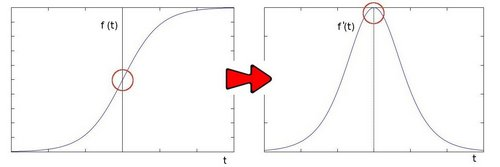
\includegraphics[width=0.7\columnwidth]{picture/LLIE/first-order derivative}
				%\captionsetup{font=scriptsize}
				\caption{
					\label{fig: first-order derivative} 
					在边缘区域,像素强度表现出“跳跃”或强度的高变化。获取强度的一阶导数,找到最大的一阶导数也就找到了像素变化最大的点,即边缘点。
				}
			\end{figure}
			
			\subsubsection{基于零穿越的边缘检测方法}
			
			基于零穿越:通过寻找二阶导数零穿越来寻找边界,代表算法是 Laplace 算子。
			
			\begin{figure}[htbp]
				% read manual to see what [ht] means and for other possible options
				\centering 
				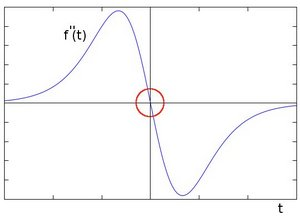
\includegraphics[width=0.6\columnwidth]{picture/LLIE/second-order derivative}
				%\captionsetup{font=scriptsize}
				\caption{
					\label{fig: second-order derivative} 
					在一阶导数的基础上再求一次导,那么此时零点就是变化最大的点,即边缘点。
				}
			\end{figure}
		
		\subsection{算子比较}
		
			\begin{table}[!htbp]
				\centering
				\small
				\caption{\label{tab: Operator comparison}
					不同算子的优缺点比较} %表格的标题
				%\resizebox{\textwidth}{!}{ %按照宽度调整调整表格大小
					\begin{tabular}{>{\centering\arraybackslash}m{2.6cm}|c}
						
						\hline
						
						\textbf{Operator} & \textbf{Comparison} \\
						
						\hline
						
						Roberts   & \makecell[l]{对具有陡峭的低噪声的图像处理效果较好,但利用 Roberts 算子提取边缘的结果是边缘比\\较粗,因此边缘定位不是很准确。}  \\ 
						Sobel     & \makecell[l]{对灰度渐变和噪声较多的图像处理效果比较好,Sobel 算子对边缘的定位比较准确。}  \\ 
						Kirsch    & \makecell[l]{对灰度渐变和噪声较多的图像处理效果较好。}   \\
						Prewitt   & \makecell[l]{对灰度渐变和噪声较多的图像处理效果较好。}   \\
						Laplacian & \makecell[l]{对图像中的阶跃性边缘点定位准确,对噪声非常敏感,丢失一部分边缘的方向信息,造成\\一些不连续的检测边缘。}  \\
						LoG		  & \makecell[l]{LoG 算子经常出现双边缘像素边界,而且该检测方法对噪声比较敏感,所以很少用 LoG \\算子检测边缘,而是用来判断边缘像素是位于图像的明区还是暗区。}  \\
						Canny     & \makecell[l]{此方法不容易受噪声的干扰,能够检测到真正的弱边缘。在 edge 函数中,最有效的边缘\\检测方法是 Canny 方法。该方法的优点在于使用两种不同的阈值分别检测强边缘和弱边\\缘,并且仅当弱边缘与强边缘相连时,才将弱边缘包含在输出图像中。因此,这种方法不\\容易被噪声“填充”,更容易检测出真正的弱边缘。}  \\
						
						\hline
						
					\end{tabular}
					%}
				\captionsetup{font=scriptsize} %设置标题字体与表格字体一致
			\end{table}

			以下是一些常见的边缘检测方法:
			
						
			\begin{itemize}
				\item[1)] 
				Roberts 边缘检测:Roberts 边缘检测算子是一种利用局部差分算子寻找边缘的算子,它在图像处理后的结果边缘不是很平滑。
				
				\item[2)]
				Sobel 边缘检测:Sobel 边缘检测算子对像素灰度值做了加权平均, 提供了较为连续的边缘方向信息。在技术上, Sobel 算子是一种利用离散性差分算子计算图像亮度梯度的近似值。
				
				\item[3)]
				Kirsch 边缘检测:Kirsch 边缘检测利用 8 个方向的核对图像进行检测,使每个像素点的结果为八个方向中响应最大的值。
				
				\item[4)]
				Prewitt算子是一种一阶微分算子的边缘检测方法,它利用像素点上下、左右邻点的灰度差,在边缘处达到极值检测边缘,去掉部分伪边缘,对噪声具有平滑作用。
				
				\item[5)]
				Laplacian边缘检测:Laplacian(拉普拉斯)算子是一种二阶导数算子,其具有旋转不变性,可以满足不同方向的图像边缘锐化(边缘检测)的要求。
				
				\item[6)]
				LoG (Laplacian of Gaussian) 边缘检测:LoG 边缘检测步骤包括先用 $n*n$ 的高斯进行平滑处理;对平滑后的图像再使用拉普拉斯算子进行边缘检测;再找出图像的零交叉点,进行边界连接。
				
				\item[7)]
				Canny边缘检测:Canny 边缘检测是一种多级别的检测方法,由 John F. Canny 于 1986 年提出。它包括五个步骤:高斯滤波、计算梯度大小和方向、非极大值抑制、双阈值处理和孤立弱边缘抑制。
				
			\end{itemize}	

	\section{方向}
	
		边缘检测\footnote{人类视觉系统对边缘高度敏感,保留结构信息对图像重建任务的性能至关重要。定义边缘可以通过学习区分黑暗区域的不同物体来指导增强过程,而不仅仅是识别低光区域。通过保留图像中的颜色和结构属性,这使得物体之间的可见性更好。}:
		
		\begin{itemize}
			\item[(1)] 
			手工设计各种滤波器来生成边缘图。
			
			\item[(2)]
			根据人类设计的特征使用数据驱动模型来预测边缘(随机决策森林来学习边缘斑块)
			
			\item[(3)]
			深度学习方法从原始数据中学习复杂的特征表示端到端边缘检测模型。
		\end{itemize}	
	
		\begin{figure}[htbp]
			% read manual to see what [ht] means and for other possible options
			\centering 
			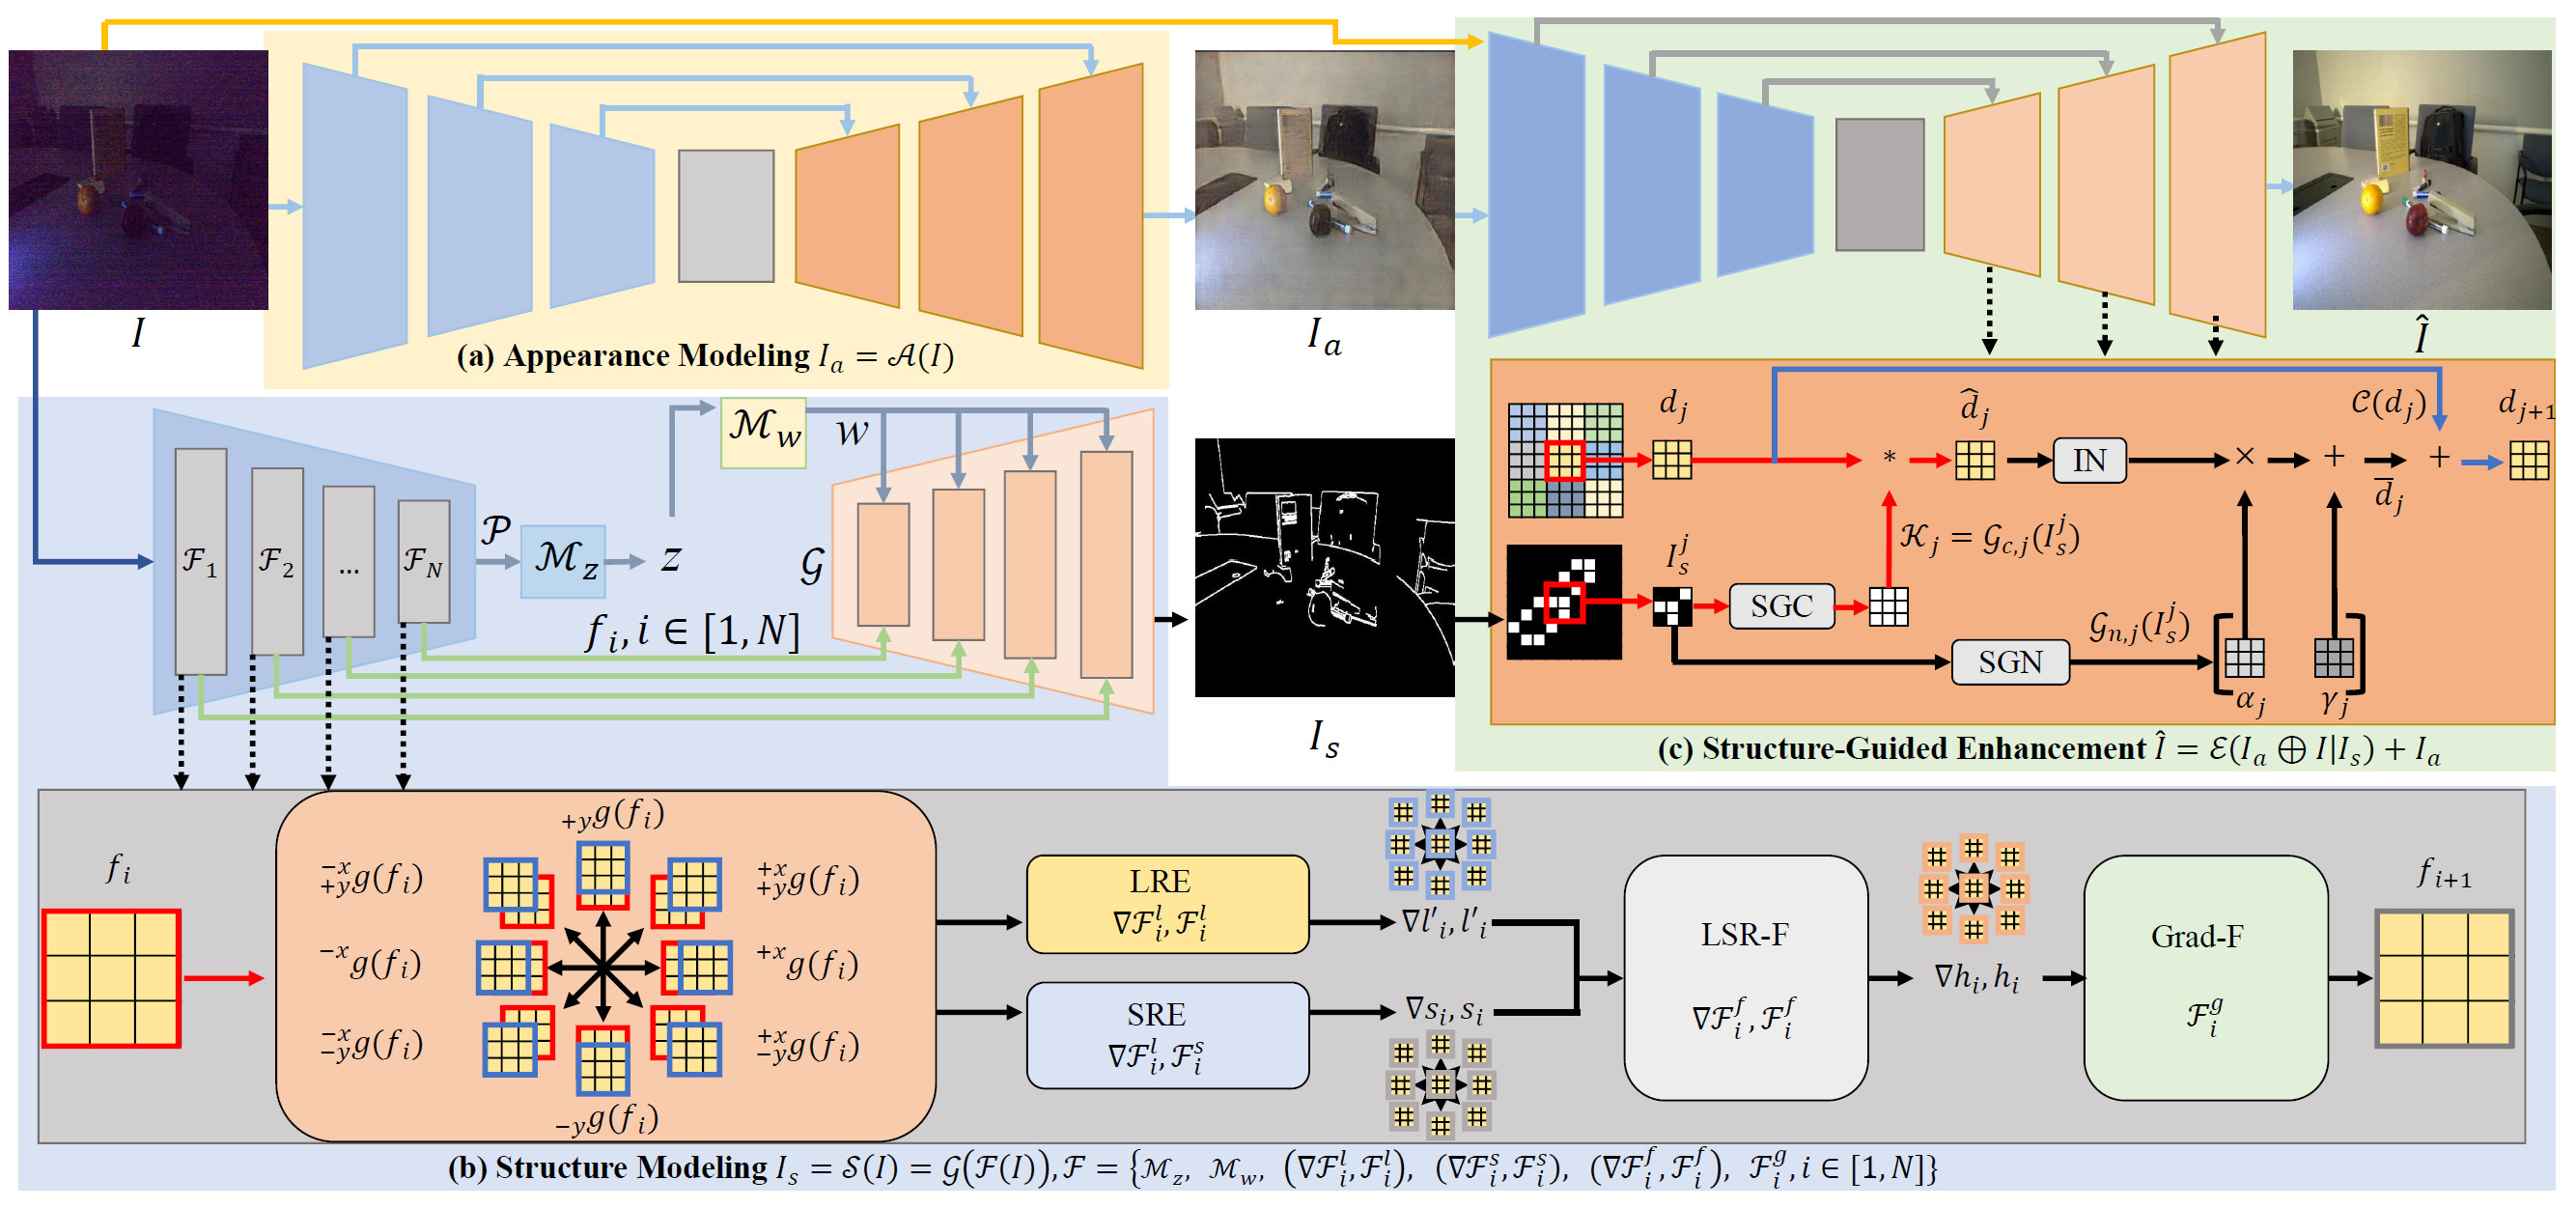
\includegraphics[width=\columnwidth]{picture/LLIE/Overview}
			%\captionsetup{font=scriptsize}
			\caption{
				\label{fig: Overview} 
				The overview of our framework with explicit appearance modeling $\mathcal{A}$, structure modeling $\mathcal{S}$, and SGEM $\mathcal{E}$. The supervision for $I_a$ and $\widehat{I}$ is the normal-light image $\bar{I}$, and for $I_s$ is the edge $\bar{I}_s$ extracted from $\bar{I}$. The overall framework can be trained end-to-end.
			}
		\end{figure}
		
		\cite{rana2021edge}与\cite{zhu2020eemefn}在暗区域中加入敏感边缘先验可以降低优化外观重构时的不适定程度。

		这个边缘检测的思想目前的文献调研显示只集中在边缘检测和外观指导图像恢复,没有考虑和图像的色彩结合,以及恢复出来的图像还是有明显噪点。
		
		\textbf{问题}:目前的文献调研结果显示,采用边缘检测思想指导恢复的模型,通常采用边缘图 + 初步恢复的图 Concat 之后采用单个增强网络进行恢复。该弱光图像恢复效果往往取决于最后增强网络的设计或是“初步恢复的图”中所包含的特征与真实图片特征的相似度。目前采用的初步恢复方法,一种是通过多曝光方法来获取不同曝光度下的图片,进而结合恢复网络进行初步恢复。第二种是直接通过网络进行一个弱恢复,结果具有噪点、伪影,同时色彩与真实图片存在较多差异。对于增强网络的设计,目前的方法主要采用StyleGAN和U-Net,采用 Concat 方式或是把边缘图分块当作卷积核的方式进行指导恢复。此外,获取边缘图的方式不同,一般采用边缘网络获取边缘图,Canny 和 Sobel 用作对比实验,亦或者是辅助边缘网络以提高边缘网络的准确度。
		
		\textbf{创新想法}:采用不同的边缘图获取方法(需要调研),尝试基于 VGG 的方法构建一个边缘图,采用 Canny 参考对比方法。主要的恢复思路为采用边缘图 + 初步恢复的图 + 原图 Y/CB/Cr的通道信息\footnote{Y通道代表的是亮度信息 (Luma),也就是图像的明暗信息; Cb 和 Cr 通道则代表的是色度信息 (Chroma),也就是图像的色彩信息。Cb 通道表示的是蓝色分量与亮度的差值,Cr 通道表示的是红色分量与亮度的差值。}。对于初步恢复的图,采用一种复合型 CNN + Transformer 网络以获取弱光图像的长距离和短距离特征,以期从弱光图像中获取更多的图像特征,然后进行特定的特征融合后,获得初步恢复的图。增强网络部分暂时没有想法。
		
%%%%%%%%%%%%%%%%%%%%%%%%%%%%%%%%%%%%%%%%%%%%%%%%%%%%%%%%%%%%%%%%%%%%%%%%%%%%%%%%%%%%%%%%%%%%%%%%%%%%
%%%%%%%%%%%%%%%%%%%%%%%%%%%%%%%%%%%%%%%%%%%%%%%%%%%%%%%%%%%%%%%%%%%%%%%%%%%%%%%%%%%%%%%%%%%%%%%%%%%%
%%                                                                                                %% 
%%								          Paper reading                                           %%
%%                                                                                                %%
%%%%%%%%%%%%%%%%%%%%%%%%%%%%%%%%%%%%%%%%%%%%%%%%%%%%%%%%%%%%%%%%%%%%%%%%%%%%%%%%%%%%%%%%%%%%%%%%%%%%
%%%%%%%%%%%%%%%%%%%%%%%%%%%%%%%%%%%%%%%%%%%%%%%%%%%%%%%%%%%%%%%%%%%%%%%%%%%%%%%%%%%%%%%%%%%%%%%%%%%%	

	
	\part{Paper Reading}
	
	\section{LLIE}
		
		\subsection{(2020.4)EEMEFN: Low-Light Image Enhancement via Edge-Enhanced Multi-Exposure Fusion Network}
		
		\paragraph{EEMEFN:基于边缘增强多曝光融合网络的弱光图像增强}
		
		\paragraph{(AAAI 2020) doi: doi.org/10.1609/aaai.v34i07.7013}
		
			\subsubsection{Research Background}
			
			现有的方法主要存在三个问题:
			
			\begin{itemize}
				\item[(1)] 
				低光图像通常具有高对比度。现有的方法可能无法在极暗或极亮的区域恢复图像细节;
				
				\item[(2)]
				现有方法不能精确校正弱光图像的颜色;
				
				\item[(3)]
				当物体边缘不清晰时,像素级损失往往会模糊边缘,破坏图像细节。
				
			\end{itemize}	
			
			作者想要解决弱光图像增强中的颜色偏差,揭示暗区隐藏的信息。
			
			\subsubsection{Contribution}
			
			\begin{itemize}
				\item[(1)] 
				作者提出了一种新型的多曝光融合模块和融合块,将不同光照条件下生成的图像进行融合,从而解决高对比度和偏色问题。
				
				\item[(2)]
				作者引入边缘增强模块,增强边缘锐利、结构精细的图像。
				
			\end{itemize}	
			
			\subsubsection{Approach}
			
			作者提出了一种边缘增强多曝光融合网络 (EEMEFN) 的两阶段方法来增强极弱光图像,如 Fig. \ref{fig: EEMEFN framework} 所示, EEMEFN方法由两个部分组成:多曝光融合 (Multi-Exposure Fusion) 和边缘增强 (Edge Enhancement)。
			
			\begin{itemize}
				\item[(1)] 
				在第一阶段,作者采用多曝光融合模块 (MEF) 来解决高对比度和颜色偏差问题。作者从一张图像合成一组不同曝光时间的图像,并将不同光照条件下的良好曝光区域组合在一起,构建出精确的正光图像。通过这种方式,图像可以从极噪和低光的图像中产生具有正确颜色的逼真初始图像。
				
				\item[(2)]
				其次,引入边缘增强模块,利用边缘信息对初始图像进行细化;
				
			\end{itemize}	
			
			作者的方法可以在最小化像素损失\footnote{像素损失是一种常用的损失函数,它计算的是生成图像 (SR) 与真实高分辨率图像 (HR) 对应像素位置的值的误差。像素损失是一种常用的损失函数,它计算的是生成图像(SR)与真实高分辨率图像(HR)对应像素位置的值的误差。由于峰值信噪比 (PSNR) 的定义与像素差异高度相关,最小化像素损失可以直接最大化 PSNR。但是,像素损失实际上并没有考虑图像质量(例如,感知质量、纹理),它通常缺乏高频细节,产生过度平滑的纹理。}的情况下重建具有清晰边缘的高质量图像。
			
			\begin{figure}[htbp]
				% read manual to see what [ht] means and for other possible options
				\centering 
				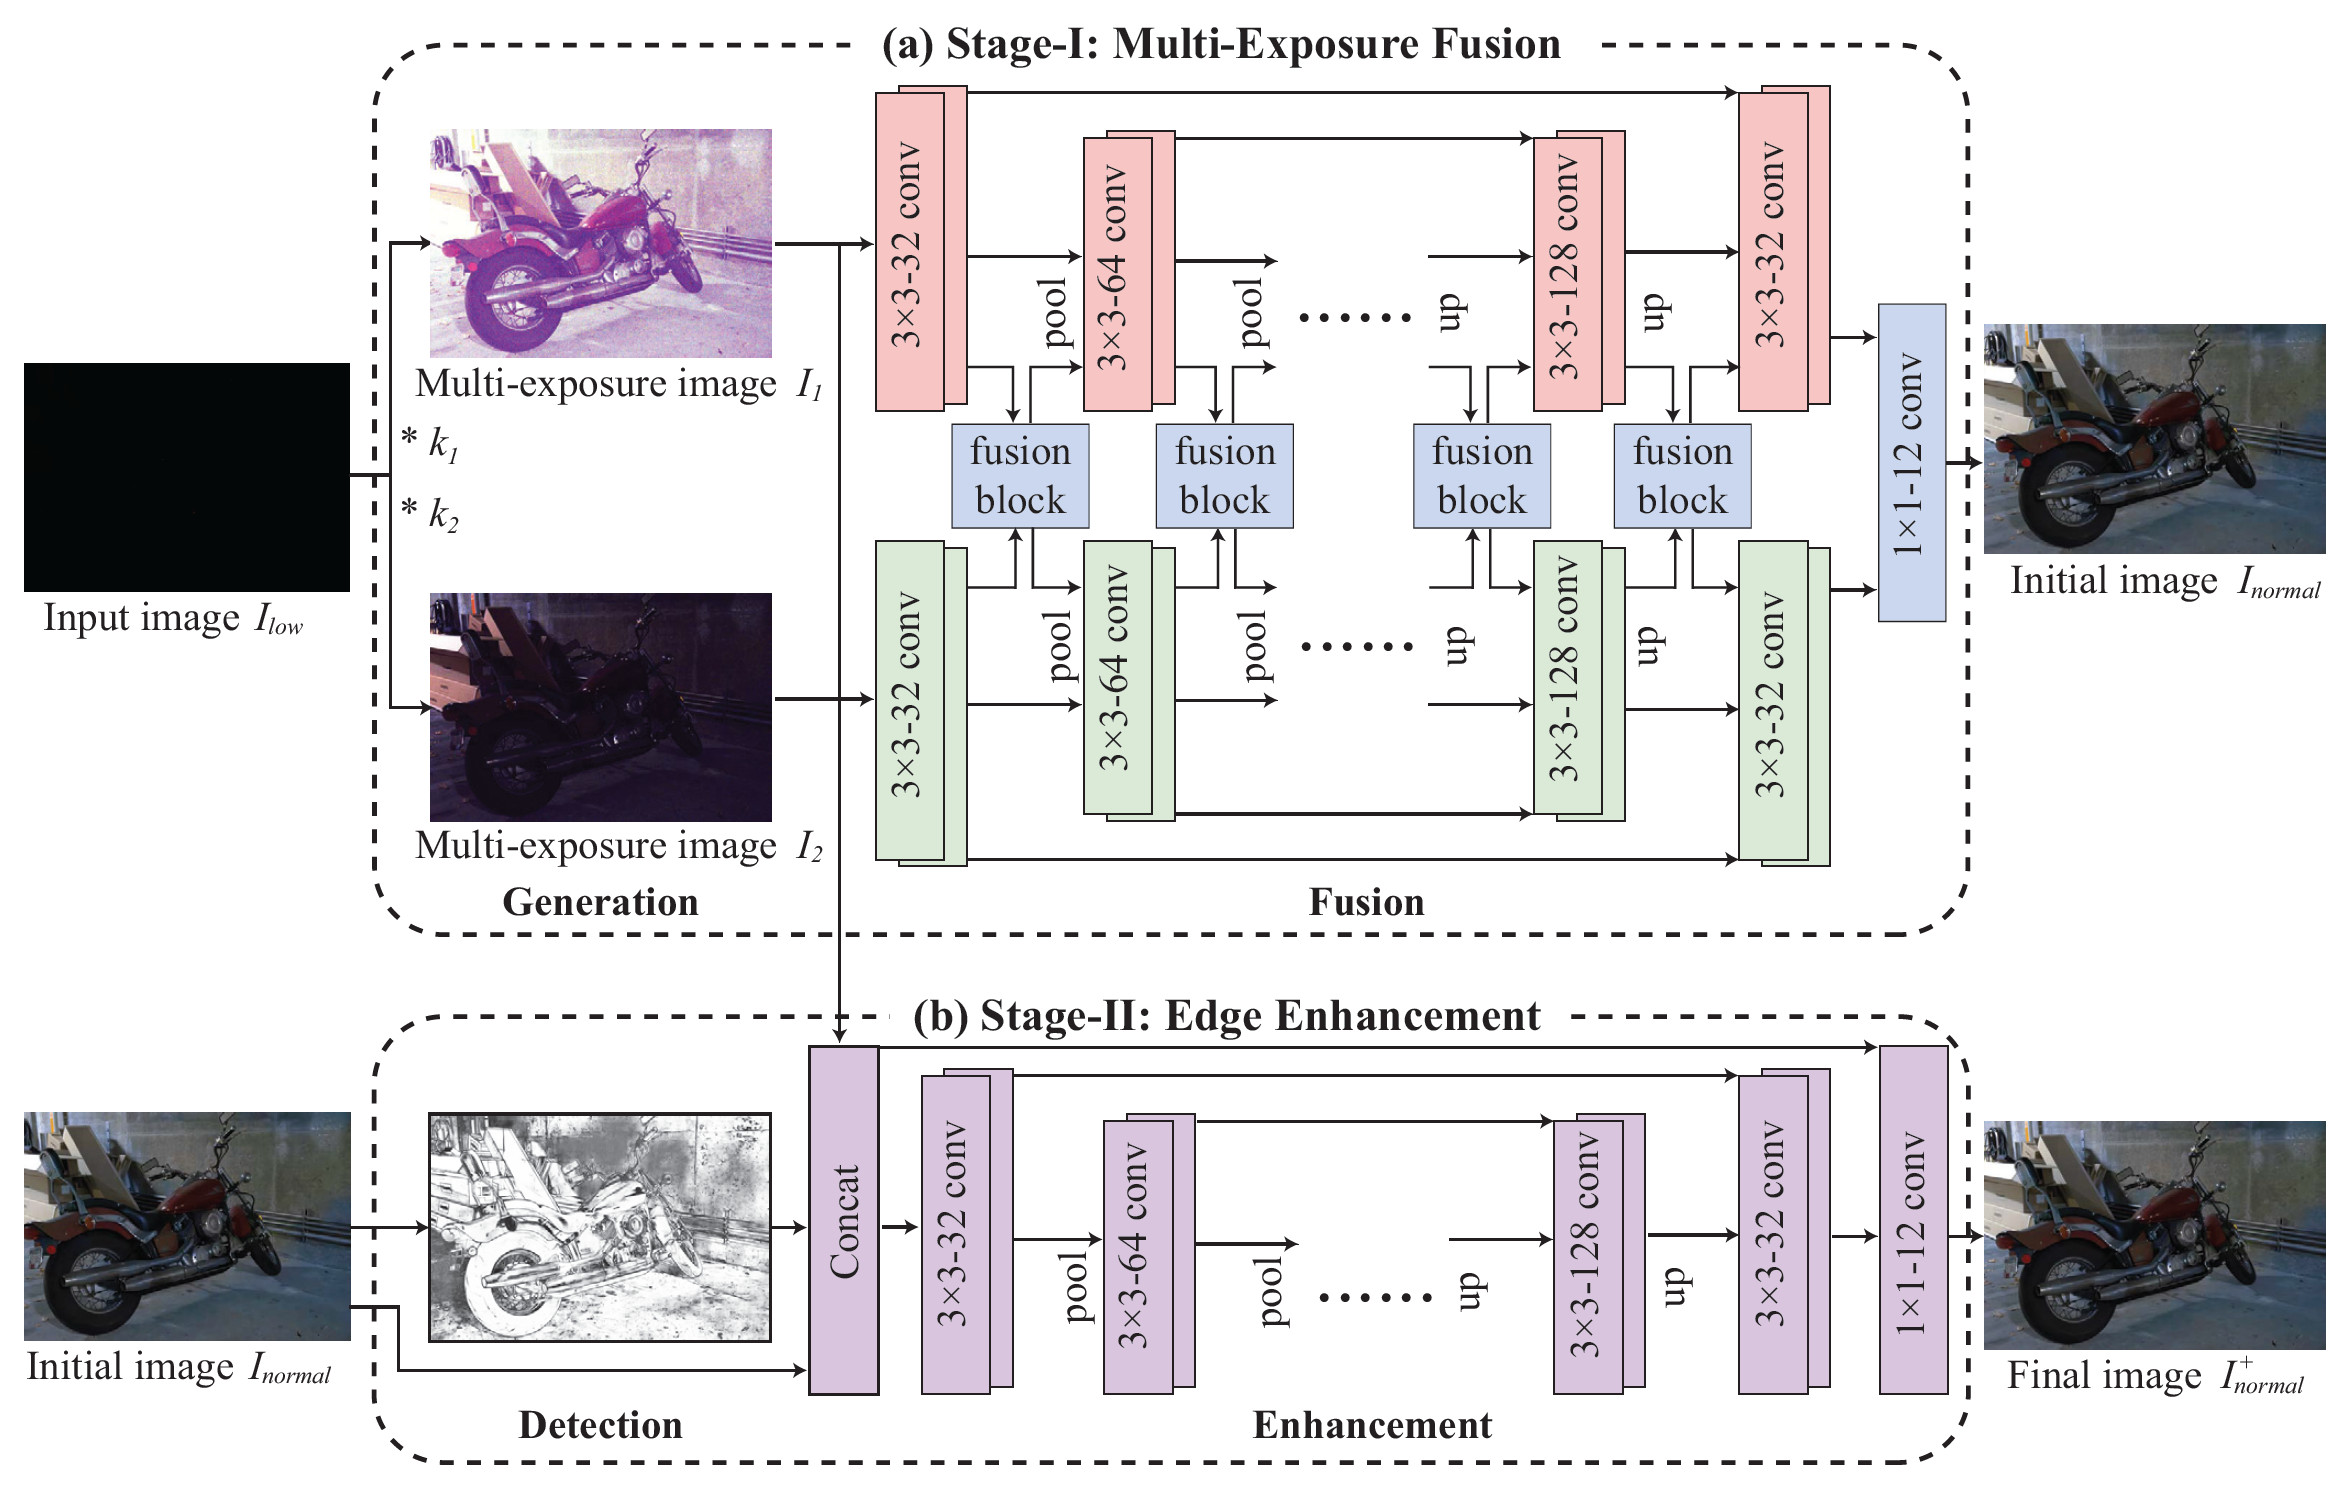
\includegraphics[width=\columnwidth]{picture/LLIE/EEMEFN/EEMEFN framework}
				%\captionsetup{font=scriptsize}
				\caption{
					\label{fig: EEMEFN framework} 
					Demonstration of our framework for low-light image enhancement. The proposed EEMEFN consists of two stages: (a) multi-exposure fusion and (b) edge enhancement. The multi-exposure fusion module first generates several images in different light conditions and then fuses images into one high-quality initial image. The edge enhancement module obtains an edge map from the initial image and combines edge information to yield the final enhanced image.
				}
			\end{figure}
			
			\paragraph{Multi-Exposure Fusion}
			
			多曝光融合模块 (MEF) 将不同曝光比的图像融合为一幅高质量的初始图像(如 Fig. \ref{fig: EEMEFN framework} 所示)。其主要步骤为\textbf{通过缩放不同放大比的像素值}来生成一组不同光照条件下的多曝光图像。合成图像可以在原始图像曝光不足的区域中曝光良好。
			
			首先,每张图片由具有相同架构的 U-Net 分支进行处理,作者在 U-Net分支中添加了跳过连接\footnote{在 U-Net 中,跳过连接 (Skip connection) 的作用主要是将底层的位置信息与深层的语义信息相融合,跳过连接可以帮助网络在每一级的上采样过程中,将编码器对应位置的特征图在通道上进行融合。通过底层特征与高层特征的融合,网络能够保留更多高层特征图蕴含的高分辨率细节信息,从而提高了图像分割精度},可以在不同尺度上重建细节。
			
			\begin{figure}[htbp]
				% read manual to see what [ht] means and for other possible options
				\centering 
				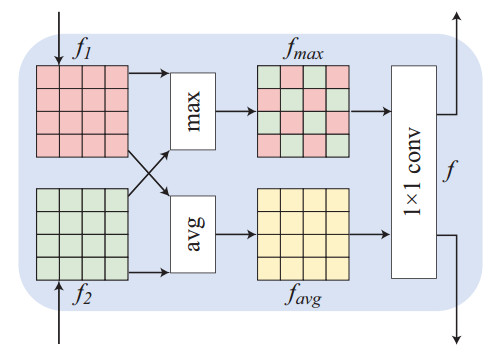
\includegraphics[width=0.45\columnwidth]{picture/LLIE/EEMEFN/Fusion block}
				%\captionsetup{font=scriptsize}
				\caption{
					\label{fig: Fusion block} 
					The architecture of the proposed fusion block.
				}
			\end{figure}
			
			其次,作者提出了融合块,将不同分支获得的图像特征结合起来,以互补的方式充分利用有价值的信息(如 Fig. \ref{fig: EEMEFN framework}(a) 所示)。融合块 (Fusion block) 建立了一种排列不变技术,特征之间有更多的聚合操作。因此,MEF 模块可以从黑暗区域恢复准确的图像细节,使颜色分布更接近真实值。每个融合块取 $N$ 个图像特征 $f_1, f_2, \ldots, f_N \in \mathbb{R}^{c \times hw}$ 作为输入,对 $N$ 个分支进行最大 (max) 和平均 (avg) 运算,提取有价值的信息。
			
			\begin{equation}
				\begin{aligned}
					f_{max} = \max (f_1, f_2, \ldots, f_N) , \\
					f_{avg} = \left( f_1 + f_2 + \ldots , f_N\right) / N
				\end{aligned}
				\label{eq: max and avg}
			\end{equation}
			
			然后,将特征 $f_{max}$ 和 $f_{avg}$ 变换到输入特征空间中,并将它们返回到每个分支中。
			
			\begin{equation}
				\begin{aligned}
					f = W * \left[f_{max}, f_{avg}\right], f \in \mathbb{R}^{c \times hw}, W \in \mathbb{R}^{c \times 2c}
				\end{aligned}
				\label{eq: fusion}
			\end{equation}
			
			其中 $\left[ \cdot , \ \cdot \right]$ 表示拼接操作,$f$ 为输出特征,$W$ 为学习到的权值矩阵。
			
			最后,将所有分支的最后一个特征连接在一起,并馈送到 $1 \times 1$ 的 Conv 层中,通过对所有分支的联合学习产生期望的输出\footnote{这里描述了一种常见的深度学习模型设计策略:通过多个并行处理分支和 $1 \times 1$ 卷积层来提取和融合特征,然后通过训练来优化模型参数,使得模型输出尽可能接近期望输出。}。
			
			\paragraph{Edge Enhancement}
			
			边缘增强 (EE) 模块的目的是增强 MEF 模块生成的初始图像。如 Fig. \ref{fig: EEMEFN framework}(b) 所示,EE 模块包括两个主要步骤:检测 (Detection) 和增强 (Enhancement) 。在检测步骤中,作者首先从初始图像生成边缘映射,而不是从输入图像生成边缘映射。输入图像和多曝光图像噪声较大,使得边缘提取具有挑战性。MEF 模块有效地去除噪声,并生成具有精确边缘映射的清晰正光图像。在增强步骤中,EE 模块利用边缘信息增强初始图像。借助预测的边缘图,EE 模块可以生成更光滑、颜色一致的物体表面,并恢复丰富的纹理和锐利的边缘。
				\subparagraph{Detection}
				
				作者使用边缘检测网络来预测 $I_{normal}$ 的异常的边缘 $E \in \mathbb{R}^{H \times W \times 1}$ ,其中 $E = Detection(I_{normal})$。然后利用边缘信息指导高质量图像的重建。边缘检测网络由五个阶段组成,每个阶段都利用卷积层的所有激活来执行逐像素预测 $(E1, E2, E3, E4, E5)$。最后,采用融合层对各阶段的 CNN 特征进行精心组合。作者提出的边缘检测网络可以得到精确的边缘图 E。此外,作者使用 Canny 边缘检测器来作为对照。
				
				\subparagraph{Enhancement}
				
				增强步骤采用 U-Net 结构\footnote{从Fig. \ref{fig: EEMEFN framework}(b)中可以看出,增强器 (Enhancer) 利用了图像中的全局像素信息和边缘图中的局部边缘信息。},取多曝光图像 $I = \left\{I_1, I_2, \ldots , I_N\right\}$,初始图像 $I_{normal}$ 和边缘映射 E 作为输入,将这些图片进行积分,得到最终增强的图片 $I_{normal}^{+}$
				
				\begin{equation}
					\begin{aligned}
						I_{normal}^{+} = Enhancement(I, I_{normal}, E)
					\end{aligned}
					\label{eq: fusion}
				\end{equation}
			
			\subsubsection{Future}
		
			-
			
		\subsection{(2021.5)Edge guided low-light image enhancement}
			
		\paragraph{边缘引导的低光图像增强 }
			
		\paragraph{(2021 5th International Conference on Intelligent Computing and Control Systems (ICICCS)) doi: 10.1109/ICICCS51141.2021.9432150}
			
			\subsubsection{Research Background}
				
			LLIE 单个网络泛化性低,但在不传递任何附加信息的情况下,简单地泛化网络来学习变换低光图像可能会削弱其增强能力。弱光图像增强的一个问题是无法获得成对数据。为了克服这一限制,通过多张曝光良好的图片来合成逼近真实照片。为了提高低光图像的质量,需要考虑提高对比度,照明,保持颜色的准确性和消除噪声。
			
			Retinex 模型的局限性在于缺乏准确分解图像的方法。即使使用现有的方法,也很难分解曝光不足的图像,因为它通常会导致伪影和其他失真。基于去雾的方法也被用于增强曝光不足的图像,但这些方法往往存在噪声和模糊的问题,往往导致过度增强的结果。
			
			\subsubsection{Contribution}
			
			作者提出了一种由 EdgeNet 和 EnhanceNet 组成的新型深度学习架构来解决弱光图像增强问题。
			
			作者使用 EdgeNet 首先从低光图像中过滤边缘,因为它们会出现在它的格式良好的对应图像中,并将此信息与低光图像结合起来进行增强过程。
			
			EnhanceNet 反复使用上采样和下采样块的组合,从局部到全局逐渐提取特征,并消除伪影和噪声。提取的信息通过跳过连接保存在整个网络中。
				
			\subsubsection{Approach}
			
			\paragraph{EdgeNet}
			
			EdgeNet 利用改进的 U-Net 来预测低光照图像中出现的边缘。这是通过使用 Sobel 边缘检测来识别真实图像中的边缘,并训练它从相应的低光图像中预测这些边缘来实现的。
			
			\begin{figure}[htbp]
				% read manual to see what [ht] means and for other possible options
				\centering 
				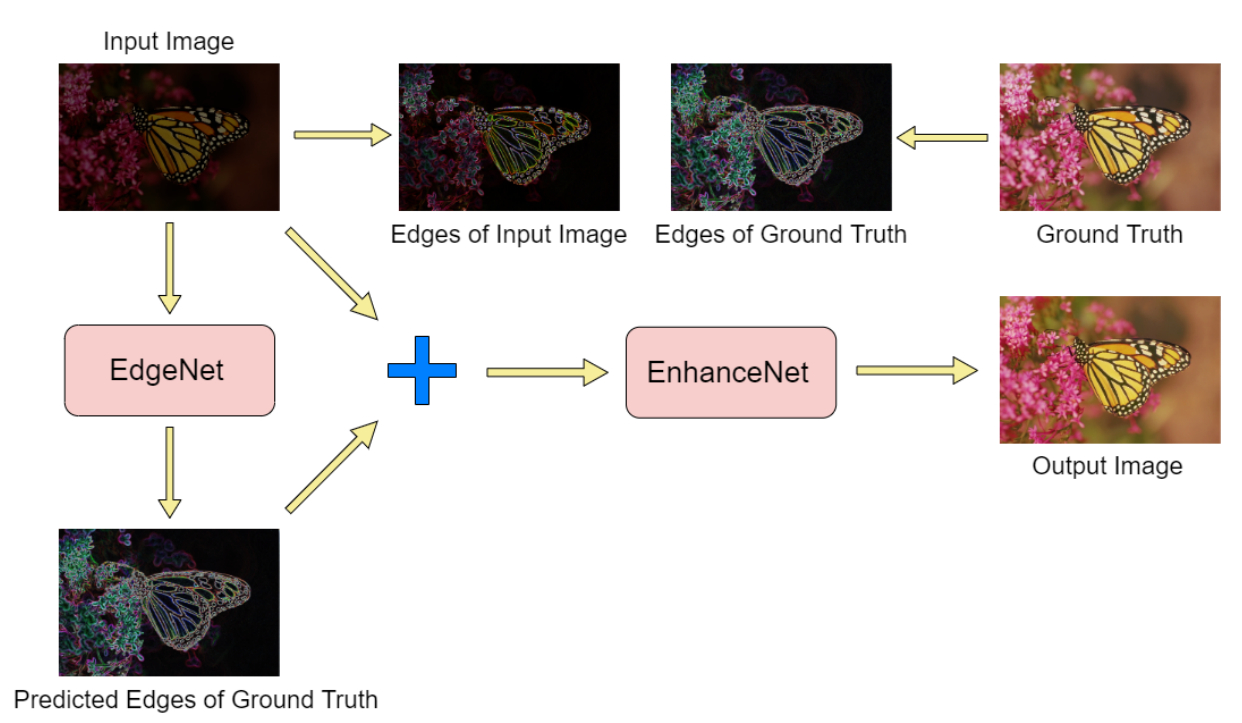
\includegraphics[width=0.6\columnwidth]{picture/LLIE/EdgeNet/Archtecture workflow}
				%\captionsetup{font=scriptsize}
				\caption{
					\label{fig: Archtecture workflow} 
					Architecture Workflow.
				}
			\end{figure}
			
			\paragraph{EnhanceNet}
			
			EnhanceNet 是一个端到端的全卷积网络,负责使用 EdgeNet 预测的边缘从输入图像中重建目标图像 (如Fig .\ref{fig: EnhanceNet})。EnhanceNet 利用网络的深层特性来预测高级特征,并使用跳过连接来维持整个网络的梯度。EnhanceNet 与其他架构相区别的一个关键特征是重复使用增强块 (如Fig .\ref{fig: Enhancement Block})。
			
			\begin{figure}[htbp]
				% read manual to see what [ht] means and for other possible options
				\centering 
				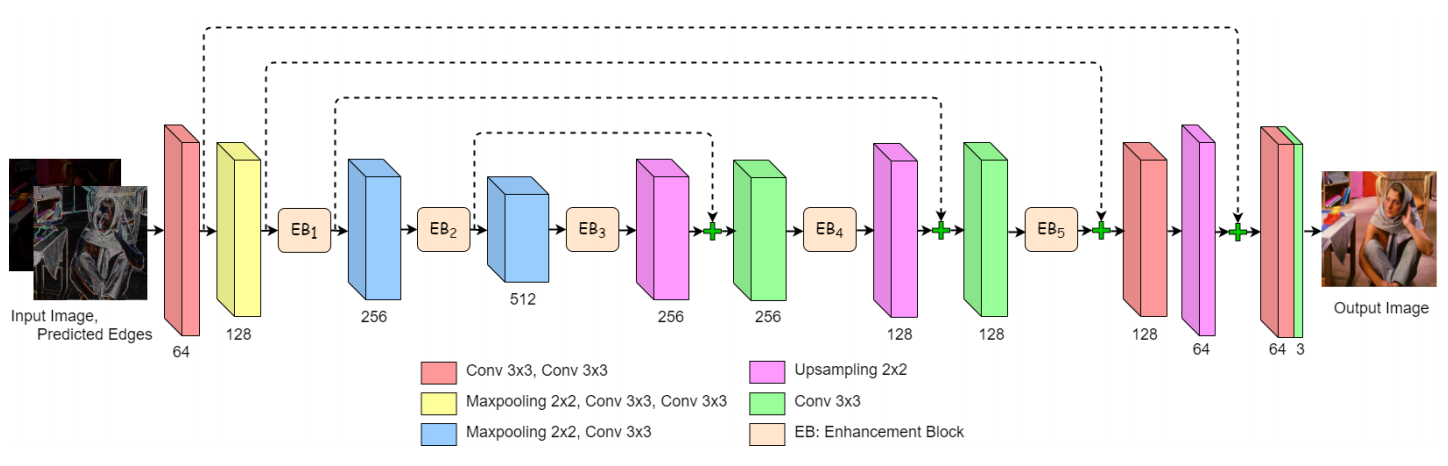
\includegraphics[width=\columnwidth]{picture/LLIE/EdgeNet/EnhanceNet}
				%\captionsetup{font=scriptsize}
				\caption{
					\label{fig: EnhanceNet} 
					EnhanceNet.
				}
			\end{figure}
						
			\begin{figure}[htbp] 
				% read manual to see what [ht] means and for other possible options
				\centering 				
				\begin{subfigure}{0.4\textwidth}
					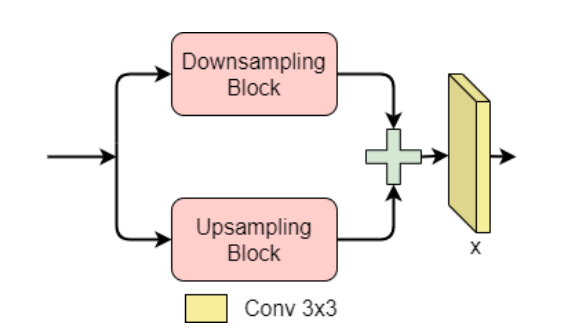
\includegraphics[width=\linewidth]{picture/LLIE/EdgeNet/Enhancement Block}
					\captionsetup{font=scriptsize}
					\caption{Enhancement Block}
					\label{fig: Enhancement Block}
				\end{subfigure}
				\begin{subfigure}{0.4\textwidth}
					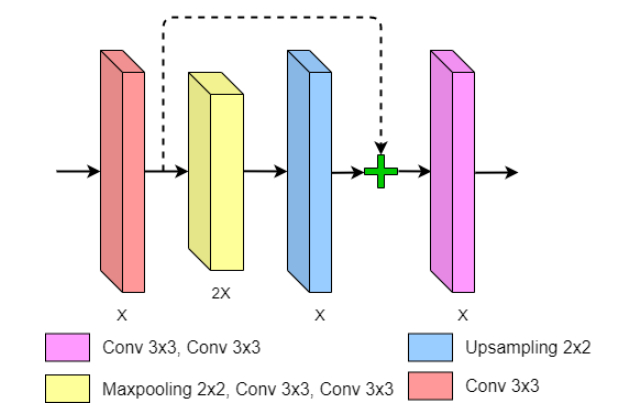
\includegraphics[width=\linewidth]{picture/LLIE/EdgeNet/Downsampling Block}
					\captionsetup{font=scriptsize}
					\caption{Downsampling Block}
					\label{fig: Downsampling Block}
				\end{subfigure}
				\captionsetup{font=scriptsize}
				\caption{
					\label{fig: Enhancement Block and Downsampling Block}
					Enhancement Block and Downsampling Block.
				}
			\end{figure}
			
			增强块 (Enhancement Block) \footnote{一种深度学习模型设计策略:通过下采样提取显著特征,通过上采样和跳过连接恢复图像细节,并避免棋盘效应。这种设计策略在许多领域都有广泛的应用。}的目的是减少中间激活产生的噪声并提取特征。增强块由上采样 (Upsampling) 和下采样 (Downsampling) 块组成,将这些次级块并行应用于其输入,并通过卷积层传递上采样和下采样的串联结果。
			
			上采样 (Upsampling) 块 (Fig .\ref{fig: Enhancement Block}):对图像进行超分辨率并减少噪声,然后将超分辨率图像降至原始尺寸,从而有效地降低噪声。使用转置卷积运算来实现超分辨率。一个关键方法是作者避免使用最大池化层,而是使用步幅为 2 的卷积层,以便通过考虑像素周围的信息来智能的减小尺寸\footnote{一种深度学习模型中的设计策略:\textbf{使用步幅为2的卷积层代替最大池化层,可以在减小特征图尺寸的同时保留更多的信息,从而提高模型的性能。}在 CNN 中,最大池化层 (Max Pooling Layer) 常被用来减小特征图的尺寸,即进行下采样。最大池化层的工作原理是在其接收域内选取最大的值作为输出。然而,这种操作可能会丢失一些重要的信息。相比之下,步幅为 2 的卷积层可以在减小特征图尺寸的同时,考虑到像素周围的信息。步幅为 2 意味着卷积核在输入特征图上移动时,每次移动2个像素。这样,输出特征图的尺寸会减半,达到了和最大池化层相同的下采样效果。但与最大池化层不同的是,卷积层在进行下采样的同时,还会考虑到像素周围的信息,并通过训练学习到更复杂的特征表示。}。
			
			下采样 (Downsampling) 块 (Fig. \ref{fig: Downsampling Block}):下采样块\footnote{下采样一般用(如最大池化或步幅为2的卷积)来减小特征图的尺寸,同时提取更抽象和显著的特征。这样可以减少计算量,同时增加模型的感受野,使模型能够捕获到更大范围内的信息。}从输入中提取显著特征,通过减小图像的大小并将其传递到更密集的卷积层。在增加维数的同时,通过上采样和卷积操作,可以考虑周围高层信息和避免棋盘效应\footnote{棋盘效应 (Checkerboard Artifacts) 是在图像处理中,特别是在使用转置卷积(也称为反卷积)进行上采样时可能出现的一种现象。棋盘效应的产生主要是由于转置卷积操作中的“不均匀重叠” (Uneven Overlap)。具体来说,当转置卷积的步长 (Stride) 大于 1 时,会在卷积前用 0 填充像素值。然后在进行卷积时,就可能出现卷积像素值差异较大的情况。例如,假设有两个相邻的输出像素,一个是由一个黑色像素和两个白色像素计算得到,另一个是由两个黑色像素和一个白色像素计算得到。这种差异会被放大,导致明暗相间的网格状,也就是“棋盘效应”}来增加维数。在增加大小之后,对块的输入使用跳过连接,以避免旧信息的丢失\footnote{使用跳过连接(Skip Connection)来融合低层和高层的信息。跳过连接可以将低层(浅层)的详细信息与高层(深层)的抽象信息相结合,从而提高模型对图像细节的捕获能力。}。
			
			\begin{itemize}
				\item[(1)] 
				Decom-Net 将输入的低光图像分解为照度和反射率。
				
				\item[(2)]
				Enhance-Net 将 Decom-Net 的输出作为输入,通过精心设计的 "Deep-Narrow" ResUnet结构来提高光照对比度,该结构可以堆叠更多的层以获得更好的非线性建模能力,并且与常用的 U-Net 相比具有显著的参数缩减。
				
				\item[(3)]
				作者将 Decom-Net 的反射率与 Enhance-Net 的照度相结合,得到增强结果。通过设计良好的网络和合理的损失函数设置,作者的方法可以在适当增强图像对比度的同时实现对噪声的抑制。
			\end{itemize}	
			
			
			
			\subsubsection{Future}
			
			-
			
		\subsection{(2019.15)Visual Cross-Image Fusion Using Deep Neural Networks for Image Edge Detection}
		
		\paragraph{利用深度神经网络进行图像边缘检测}
		
		\paragraph{(IEEE Access 2区) doi: 10.1109/ACCESS.2019.2914151}
		
			\subsubsection{Research Background}
			
			边缘检测\footnote{边缘检测在图像高级特征提取、特征描述、目标识别和图像理解等领域具有重要意义。因此,如何快速准确地定位和提取图像边缘特征信息一直是多年来研究的热点和课题之一。针对这两个问题,研究者进行了大量的研究,提出了各种边缘检测方法。这些方法大致可以分为两类,传统方法和基于深度学习的方法。}是计算机视觉的一个基本问题,有着广泛的应用,卷积神经网络 (CNN) 在许多图像边缘检测系统中称为基础组成部分。但基于CNN的边缘特征检测和提取方法,其边缘检测精度仍低于人类视觉感知,线条边缘模糊,过程耗时长。
			
			\subsubsection{Contribution}

			基于快速特征嵌入 (Caffe) 框架的卷积结构和视觉几何组 (VGG16) 模板,提出了一种基于视觉交叉融合 (VCF) 网络的高精度边缘检测器。作者提出的VCF模型分别通过参数降维和全连通层的交叉融合提取多层层次结构的特征,实现端到端的图像边缘检测。
		
		
%	\begin{table}[!htbp]
%		\centering
%		\small
%		\caption{\label{tab: Datasets comparison}
%			Comparison between classic LLIE datasets
%			and our UHD-LL dataset. ‘Number’: the number of
%			paired images. ‘Resolution’: the average resolution of the
%			dataset. ‘Noise’: low-light images contain noise. ‘Real’:
%			both low-light images and GT are acquired in real scenes.} %表格的标题
%		%\resizebox{\textwidth}{!}{ %按照宽度调整调整表格大小
%			\begin{tabular}{>{\centering\arraybackslash}m{2.6cm}|c|c|c|c}
%				
%				\hline
%				
%				\textbf{Dataset} & \textbf{Number} & \textbf{Resolution} & \textbf{Noise} & \textbf{Real} \\
%				
%				\hline
%				
%				SID(RAW) & 5094 & \makecell{4240 $\times$ 2832 \\ 6000 $\times$ 4000} & \checkmark & \checkmark \\ 
%				MIT-Adobe FiveK & 5000 & 4000 $\times$ 2500 &  &  \\ 
%				Exposure-Errors  & 24000 & 1000 $\times$ 900 &  &  \\
%				LOL & 500/789 & 600 $\times$ 400 & \checkmark & \checkmark \\
%				\textbf{UHD-LL(Ours)} & \textbf{2150} & \textbf{3840 $\times$ 2160} & \checkmark & \checkmark \\
%				
%				\hline
%				
%			\end{tabular}
%			%}
%		\captionsetup{font=scriptsize} %设置标题字体与表格字体一致
%	\end{table}
	


%	\part{Unity VR 开发计划}
%
%		\section{项目需求}
%	
%			\subsection{主菜单界面开发}
%	
%			\begin{figure}[htbp]
%				% read manual to see what [ht] means and for other possible options
%				\centering 
%				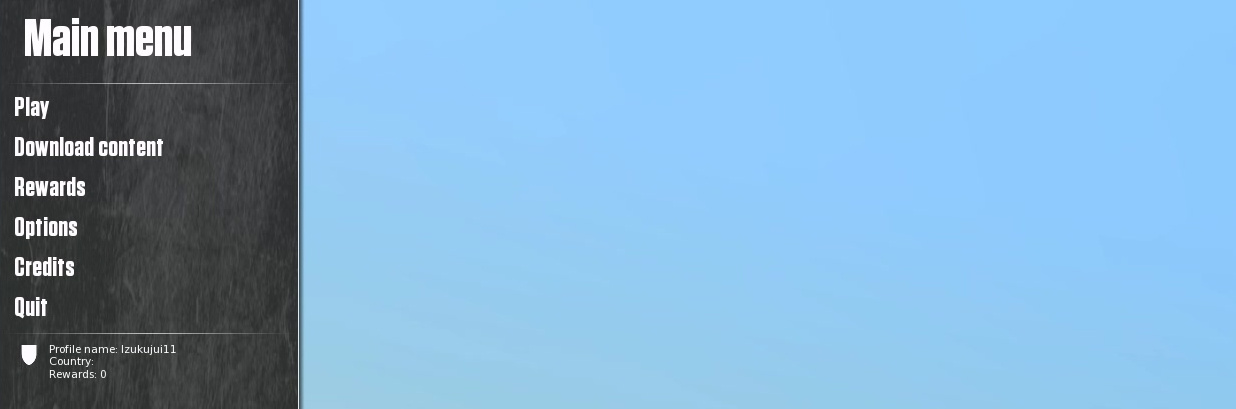
\includegraphics[width=\columnwidth]{picture/Main menu}
%				%\captionsetup{font=scriptsize}
%				\caption{
%					\label{fig: Main menu} 
%					主菜单界面。
%				}
%			\end{figure}
%			
%			启动进入游戏界面,随后进入游戏主菜单,主菜单至少需要包含 \textbf{Play},\textbf{Options}, \textbf{Quit}, 可以包含 \textbf{Credits} 和 \textbf{Rewards}。
%			
%				\subsubsection{Play}
%				
%				\begin{figure}[htbp]
%					% read manual to see what [ht] means and for other possible options
%					\centering 
%					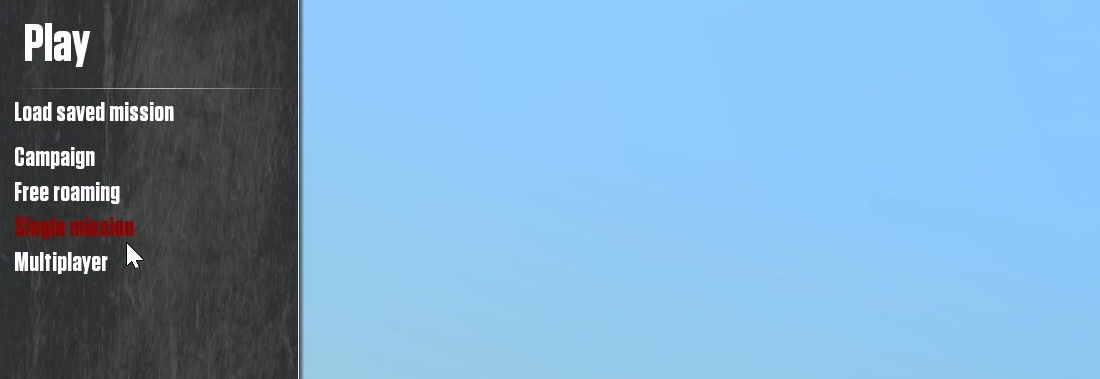
\includegraphics[width=\columnwidth]{picture/Play}
%					%\captionsetup{font=scriptsize}
%					\caption{
%						\label{fig: Play} 
%						\textbf{Play} 菜单界面。
%					}
%				\end{figure}
%				
%				通过射线选择 \textbf{Play} 进入 \textbf{Play} 菜单,\textbf{Play} 菜单至少需要包含 \textbf{Free roaming}, 可以包含 \textbf{Campaign}, \textbf{Single mission}, \textbf{Load saved mission}。玩家通过射线,选择不同的选项进入不同的游戏模式。
%				
%				\paragraph{Free roaming} 
%				
%				\textbf{Free roaming} 游戏模式赋予玩家极大的游戏自由度,进入该模式之后,玩家可以选择不同的船只与地图,同时自定义不同的海况;
%				
%				\paragraph{Campaign}
%				
%				-
%				
%				\paragraph{Single mission}
%				
%				-
%				
%				\paragraph{Multiplayer}
%				
%				-
%				
%				\paragraph{Load saved mission}
%				
%				-
%				
%				\subsubsection{Options}
%				
%					\paragraph{Controls}
%					
%					\begin{figure}[htbp]
%						% read manual to see what [ht] means and for other possible options
%						\centering 
%						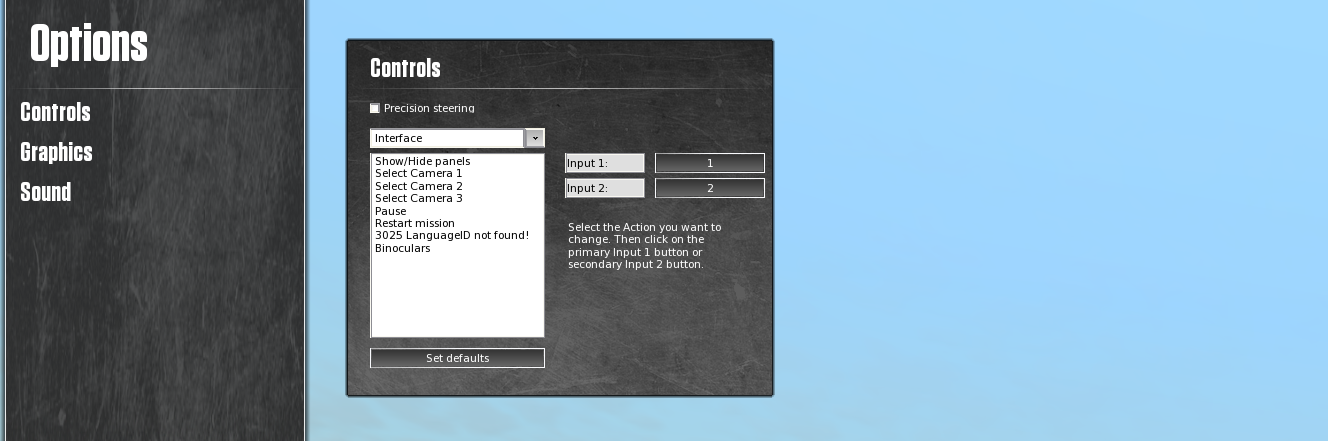
\includegraphics[width=\columnwidth]{picture/Options_Controls}
%						%\captionsetup{font=scriptsize}
%						\caption{
%							\label{fig: Options_Controls} 
%							\textbf{Controls} 选项界面。
%						}	
%					\end{figure}
%					
%					\textbf{Controls} 可以设置不同的控制模式,一种是对船面板的控制(第一人称视角),如Fig. \ref{fig: First-person perspective}所示。;另一种是以(第三人称视角)对船进行控制,并实现多种不同的第三人称视角,即多个 Camera ;最后是可以对船的控制进行自定义控制,如引擎推动开关和方向控制键。
%					
%					\begin{figure}[htbp]
%						% read manual to see what [ht] means and for other possible options
%						\centering
%						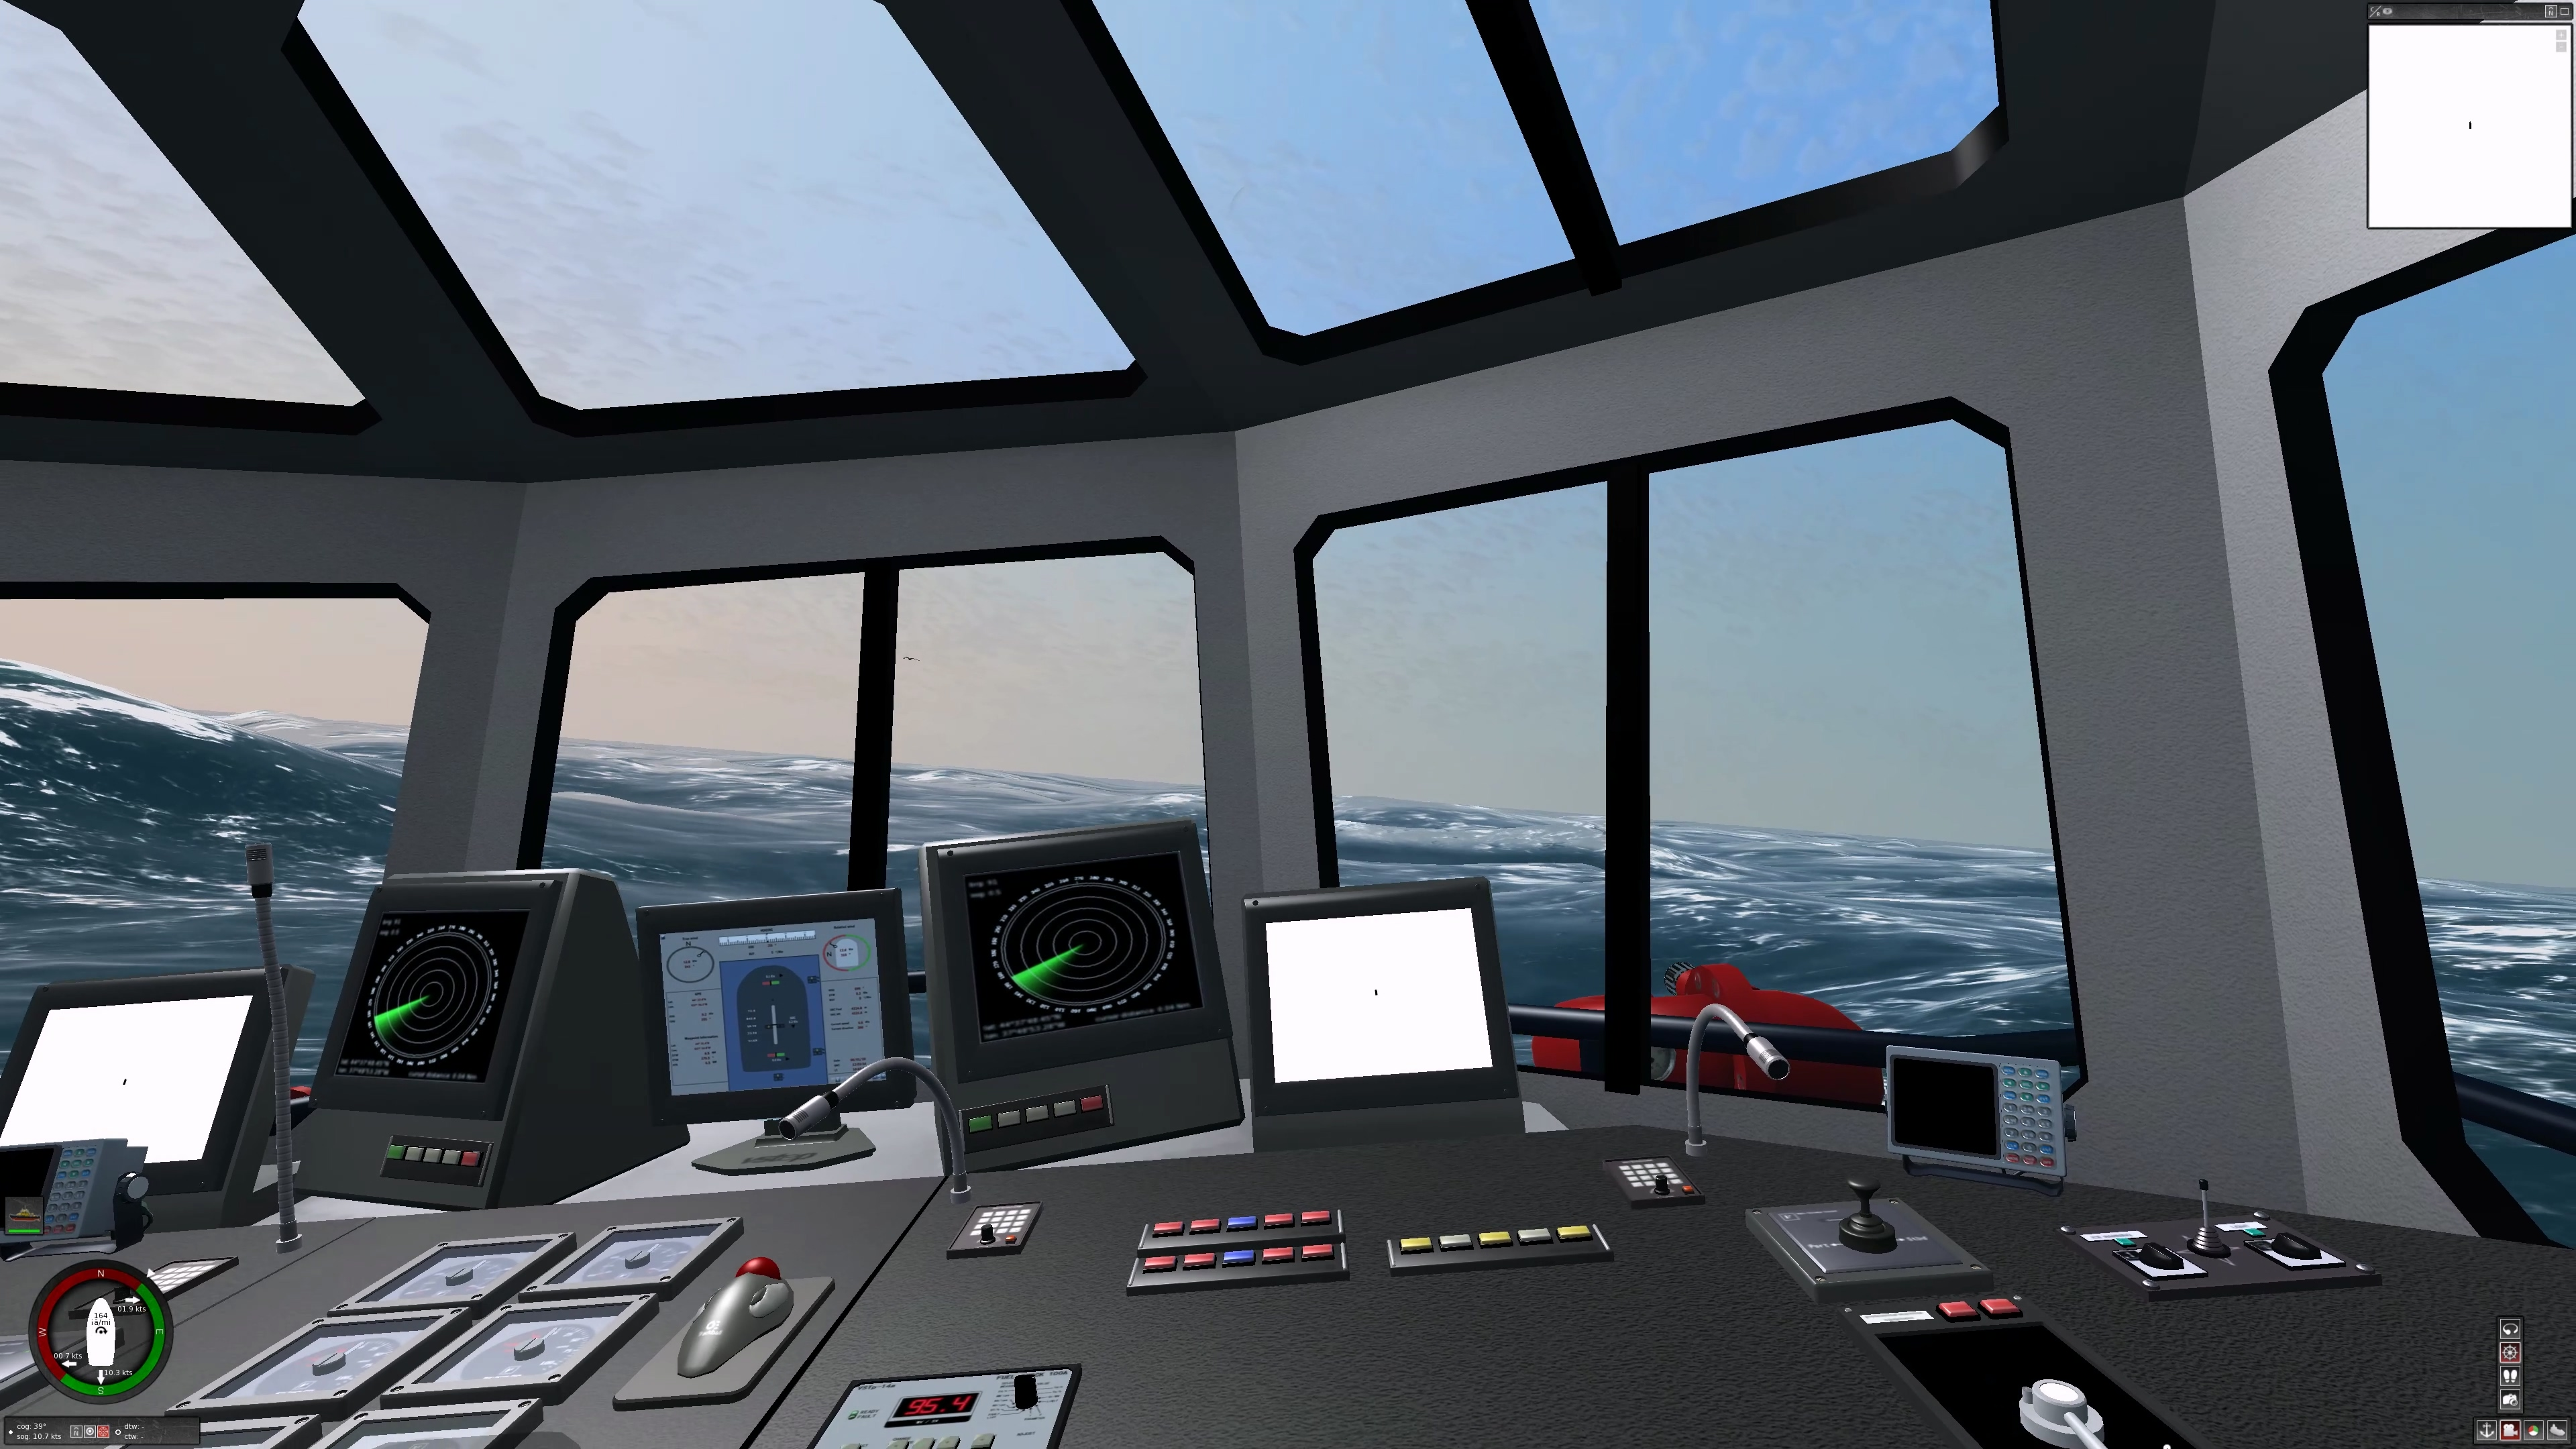
\includegraphics[width=\columnwidth]{picture/First-person perspective}
%						%\captionsetup{font=scriptsize}
%						\caption{
%							\label{fig: First-person perspective} 
%							第一人称视角游玩。
%						}	
%					\end{figure}
%					
%					
%					\paragraph{Graphics}
%					
%					\begin{figure}[htbp]
%						% read manual to see what [ht] means and for other possible options
%						\centering 
%						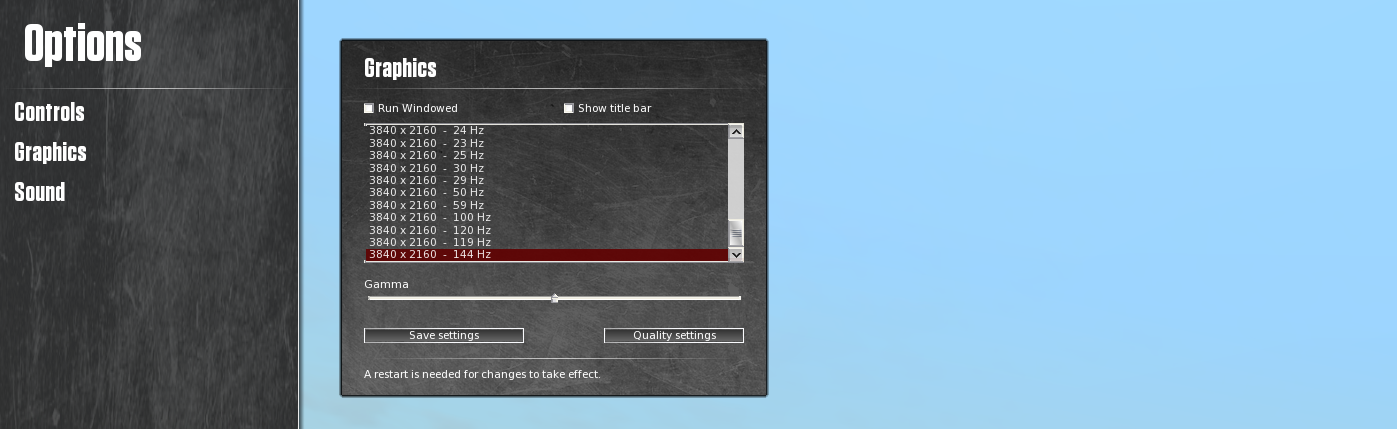
\includegraphics[width=\columnwidth]{picture/Options_Graphics}
%						%\captionsetup{font=scriptsize}
%						\caption{
%							\label{fig: Options_Graphics} 
%							\textbf{Graphics} 选项界面。
%						}	
%					\end{figure}
%					
%					\textbf{Graphics} 可以设置分辨率、是否窗口模式运行、设置刷新率和游戏渲染质量,并能够生成相应的保存的文件,每次启动时读取该保存文件。
%					
%					\paragraph{Sound}
%					
%					\begin{figure}[htbp]
%						% read manual to see what [ht] means and for other possible options
%						\centering 
%						
\includegraphics[width=\columnwidth]{picture/Options_Sound}
%						%\captionsetup{font=scriptsize}
%						\caption{
%							\label{fig: Options_Sound} 
%							\textbf{Sound} 选项界面。
%						}	
%					\end{figure}
%					
%					\textbf{Sound} 可以设置总音量(Master volume)、船只引擎的音量(Engine volume)、环境音乐的音量(Ambient volume)、界面音量( GUI volume)
%				
%				\subsubsection{Quit}
%				
%				退出游戏,即终止游戏程序运行。
%				
%				\subsubsection{Credits}
%				
%				游戏信息的展示,在主界面的滚动显示,或者是弹窗显示均可。
%				
%				\subsubsection{Rewards}
%	
%				游戏的奖杯模式,需要建立相应的任务系统,完成相应的任务之后跳杯,获得的奖杯可以在此处显示。
%	
%			\subsection{游戏模式}
%	
%				\subsubsection{Free roaming}
%				
%				\paragraph{船只模型自定义}
%				
%				\begin{figure}[htbp]
%					% read manual to see what [ht] means and for other possible options
%					\centering 
%					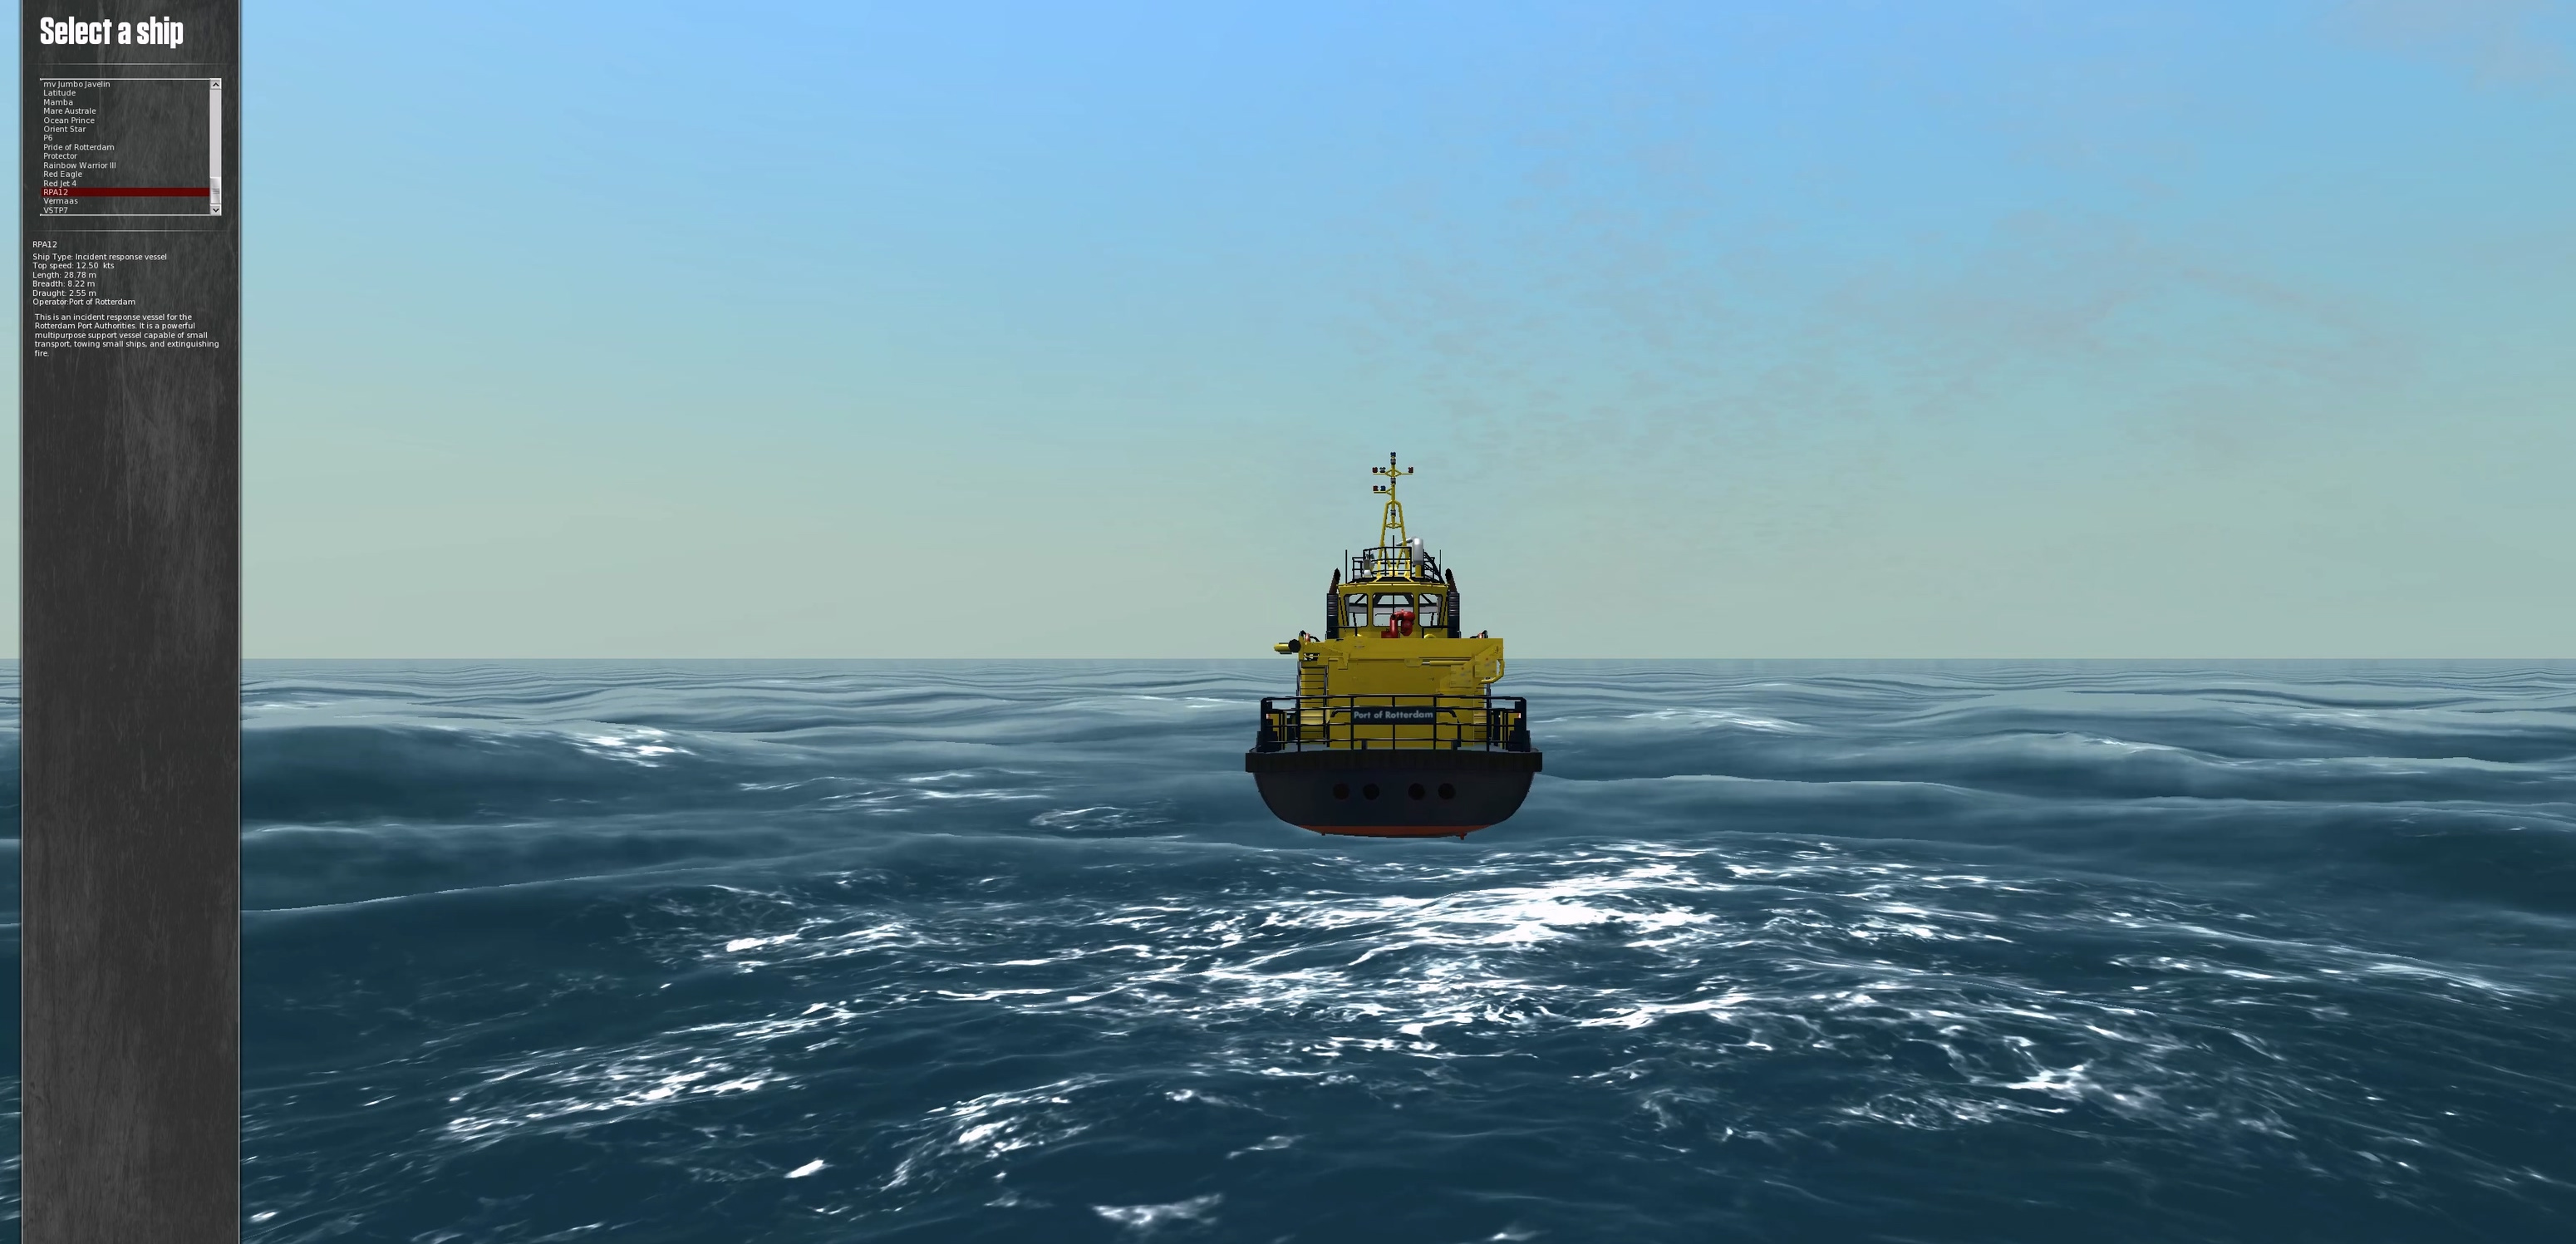
\includegraphics[width=\columnwidth]{picture/Select a ship}
%					%\captionsetup{font=scriptsize}
%					\caption{
%						\label{fig: Select a ship} 
%						船只模型选择界面。
%					}	
%				\end{figure}
%	
%				\textbf{Free roaming}下玩家可以任意进行船只选择,不同的船只会有不同的参数,如转向半径、平稳程度、马力、船只大小等会有明显区别。并且进行选择时,该船只会出现在主界面上,玩家可以直观的看到所选择的船只模型。
%				
%				\paragraph{环境自定义}
%				
%				\begin{figure}[htbp] 
%					% read manual to see what [ht] means and for other possible options
%					\centering 
%					% 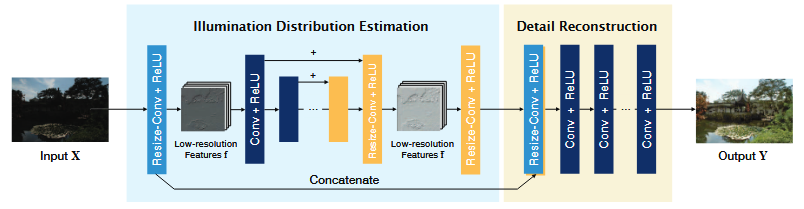
\includegraphics[width=0.8\columnwidth]{GLADNet}
%					
%					\begin{subfigure}{0.24\textwidth}
%						\includegraphics[width=\linewidth]{picture/Environment_Antarctic}
%						\captionsetup{font=scriptsize}
%						\caption{Antarctic}
%						\label{fig: Environment_Antarctic}
%					\end{subfigure}
%					\begin{subfigure}{0.24\textwidth}
%						\includegraphics[width=\linewidth]{picture/Environment_Atlantic Ocean}
%						\captionsetup{font=scriptsize}
%						\caption{Atlantic Ocean}
%						\label{fig: Environment_Atlantic Ocean}
%					\end{subfigure}
%					\begin{subfigure}{0.24\textwidth}
%						\includegraphics[width=\linewidth]{picture/Environment_Bora Bora}
%						\captionsetup{font=scriptsize}
%						\caption{Bora Bora}
%						\label{fig: Environment_Bora Bora}	
%					\end{subfigure}
%					\begin{subfigure}{0.24\textwidth}
%						\includegraphics[width=\linewidth]{picture/Environment_Dover}
%						\captionsetup{font=scriptsize}
%						\caption{Dover}
%						\label{fig: Environment_Dover}	
%					\end{subfigure} \\
%
%					\begin{subfigure}{0.24\textwidth}
%						\includegraphics[width=\linewidth]{picture/Environment_Hamburg}
%						\captionsetup{font=scriptsize}
%						\caption{Hamburg}
%						\label{fig: Environment_Hamburg}
%					\end{subfigure}
%					\begin{subfigure}{0.24\textwidth}
%						\includegraphics[width=\linewidth]{picture/Environment_Marseille}
%						\captionsetup{font=scriptsize}
%						\caption{Marseille}
%						\label{fig: Environment_Marseille}
%					\end{subfigure}
%					\begin{subfigure}{0.24\textwidth}
%						\includegraphics[width=\linewidth]{picture/Environment_New York}
%						\captionsetup{font=scriptsize}
%						\caption{New York}
%						\label{fig: Environment_New York}	
%					\end{subfigure}
%					\begin{subfigure}{0.24\textwidth}
%						\includegraphics[width=\linewidth]{picture/Environment_Padstow, Cornwall}
%						\captionsetup{font=scriptsize}
%						\caption{Padstow, Cornwall}
%						\label{fig: Environment_Padstow, Cornwall}	
%					\end{subfigure} \\
%
%					\begin{subfigure}{0.24\textwidth}
%						\includegraphics[width=\linewidth]{picture/Environment_Port of Rotterdam}
%						\captionsetup{font=scriptsize}
%						\caption{Port of Rotterdam}
%						\label{fig: Environment_Port of Rotterdam}
%					\end{subfigure}
%					\begin{subfigure}{0.24\textwidth}
%						\includegraphics[width=\linewidth]{picture/Environment_San Francisco}
%						\captionsetup{font=scriptsize}
%						\caption{San Francisco}
%						\label{fig: Environment_San Francisco}
%					\end{subfigure}
%					\begin{subfigure}{0.24\textwidth}
%						\includegraphics[width=\linewidth]{picture/Environment_Sydney}
%						\captionsetup{font=scriptsize}
%						\caption{Sydney}
%						\label{fig: Environment_Sydney}	
%					\end{subfigure}
%					\begin{subfigure}{0.24\textwidth}
%						\includegraphics[width=\linewidth]{picture/Environment_The Solent}
%						\captionsetup{font=scriptsize}
%						\caption{The Solent}
%						\label{fig: Environment_The Solent}	
%					\end{subfigure}
%					
%					\captionsetup{font=scriptsize}
%					\caption{
%						\label{fig: Environment selection}
%						在 \textbf{Free roaming} 下,玩家可以在Environment界面中自定义来自世界各地的海面环境。
%					}
%				\end{figure}
%				
%				此外,在不同的地图场景下,可以自定义船只起始出发的地点。如Fig. \ref{fig: Starting point selection}所示,在 New York 港口一共可以选择9个出发点,开始自由航行。
%				
%				\begin{figure}[htbp]
%					% read manual to see what [ht] means and for other possible options
%					\centering 
%					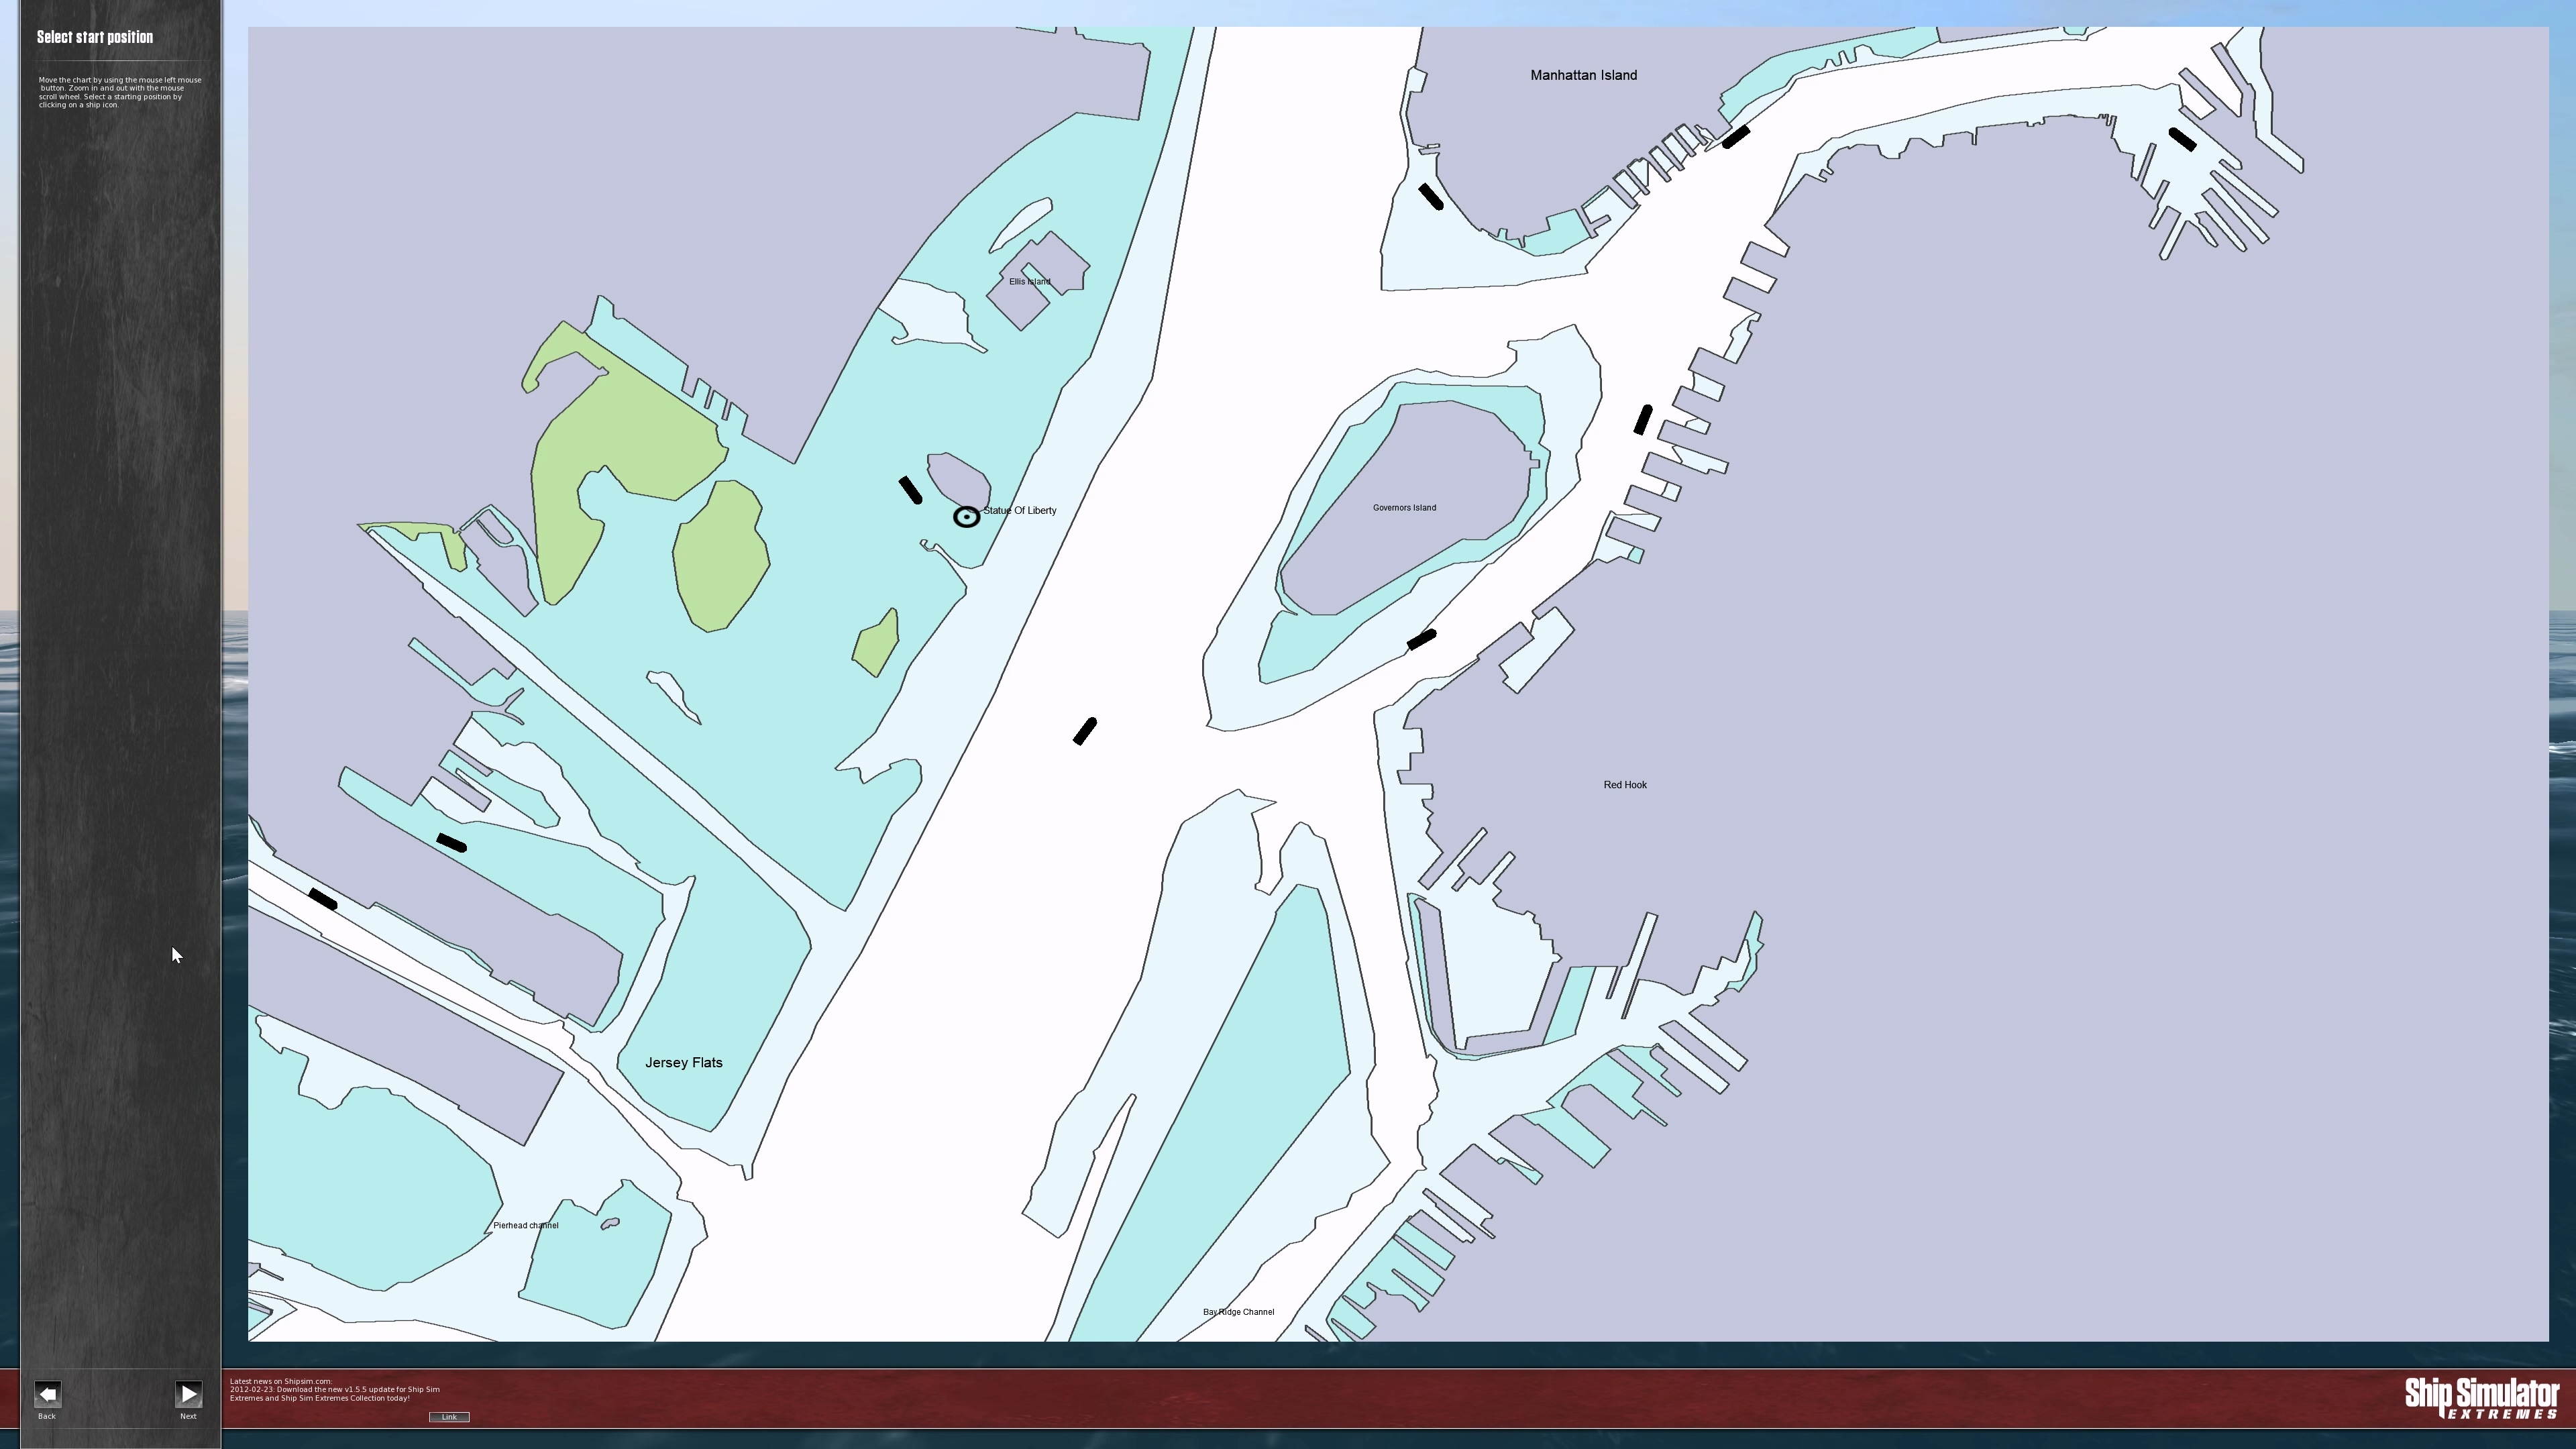
\includegraphics[width=\columnwidth]{picture/Starting point selection}
%					%\captionsetup{font=scriptsize}
%					\caption{
%						\label{fig: Starting point selection} 
%						在纽约港口环境下,船只出发地点选择。
%					}	
%				\end{figure}
%				
%				\paragraph{天气自定义}
%				
%				\begin{figure}[htbp]
%					% read manual to see what [ht] means and for other possible options
%					\centering 
%					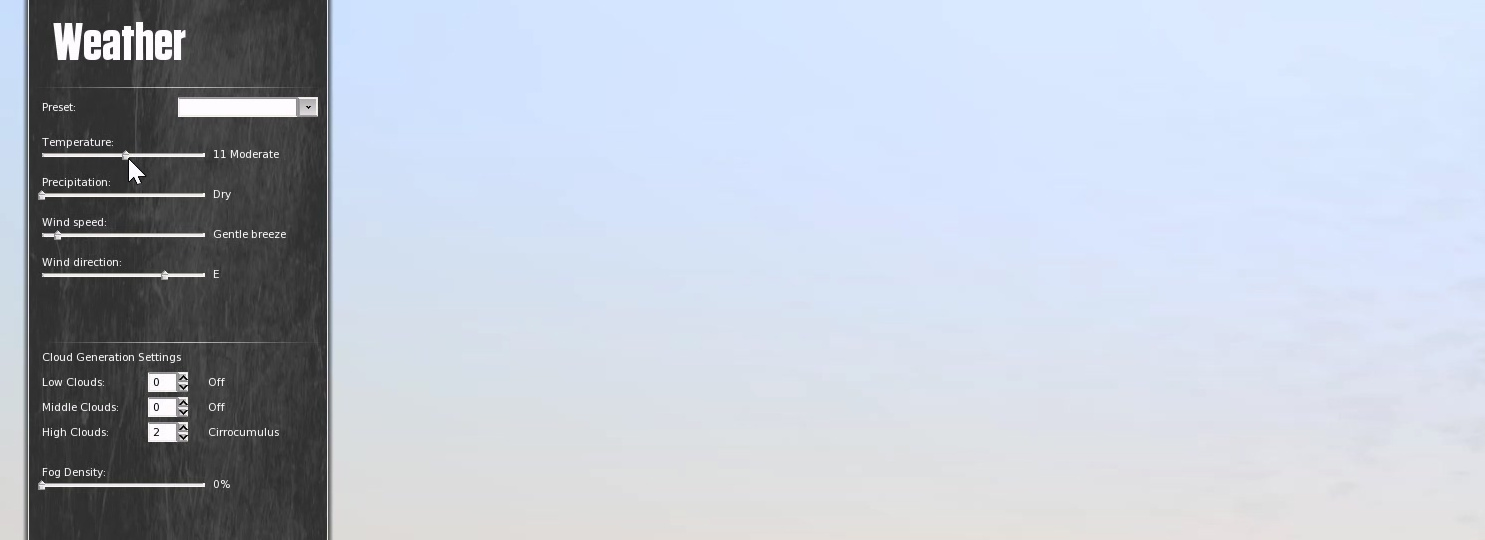
\includegraphics[width=\columnwidth]{picture/Weather}
%					%\captionsetup{font=scriptsize}
%					\caption{
%						\label{fig: Weather} 
%						天气自定义界面。
%					}	
%				\end{figure}
%				
%				\textbf{Free roaming}下玩家也可以自定义各类海洋天气,以实现不同海况下的航行。可以设置不同的 \textbf{Temperature}、\textbf{Precipitation}、 \textbf{Wind speed}、 \textbf{Wind direction} 等参数,来实现不同的海况。
%				
%				
%				主要参数有6种,每一种的定义如下:
%				\begin{itemize}
%					\item [(1)] 
%					\textbf{Temperature} 设置4个类别,共60个等级,其中 Freezing $[-20 \sim -1]$、Cold $[0 \sim 9]$、Moderate $[10 \sim 19]$、Warm $[20 \sim 29]$、Hot $[30 \sim 40]$,单位为摄氏度。
%					
%					\item [(2)]
%					\textbf{Precipitation} 设置5个等级,其中分别为 Dry, Drizzle, Rain, Heavy Rain, Cloudburst。
%					
%					\item [(3)]
%					\textbf{Wind speed} 设置13个等级,其中分别为 Calm, Light air, Light breeze, Gentle breeze, Moderate breeze, Fresh breeze, Strong breeze, Moderate gale, Fresh gale, Strong gale, Storm, Violent Storm, Hurricane。
%					
%					\item [(4)]
%					\textbf{Wind direction} 设置16个方向,其中分别为 S, SSW, SW, WSW, W, WNW, NW, NNW, N, NNE, NE, ENE, E, ESE, SE, SSE, S。
%					
%					\item [(5)]
%					\textbf{Cloud Generation Settings} 设置3个类别,分别设置 Low Clouds, Middle Clouds, High Clouds;Low Clouds 的又分为3类,其中为 0 off, 1 Nimbostratus(乱层云) 2 Cumulonimbus(积雨云); Middle Clouds 分为3类,其中为 0 off, 1 Altostratus(高层云), 2 Altocumulus(高积云); High Clouds 分为3类,其中 0 off, 1 Cirrus(卷云), 2 Cirrocumulus(卷积云)
%					
%					\item [(6)]
%					\textbf{Fog Density} 则设置为 $0 \sim 100\%$,百分比越高,能见度越差。
%				\end{itemize}
%	
%				玩家除了可以自定义天气以外,需要快捷的辅助玩家设置不同类型的天气,故引入 \textbf{Preset} 设定。\textbf{Preset} 设置了9种天气,每一种天气对应上述6种参数不同的设定,如Fig. \ref{fig: Weather}所示。9种天气为 Clear sky, Drizzle(毛毛雨), Foggy, Hail(冰雹), Light snow, Rainy, Snow storm(暴风雪), Storm, Wind\footnote{在实际的开发中,只需要开发这9种对应的天气,如果对每一种参数搭配($60 \times 5 \times 13 \times 16 \times 9 \times 100$)都开发对应的天气,这样的话,开发成本会很大。如 Clear sky 对应 27 warm, Dry, Gentle breeze, Wind E, Cirrocumulus, Fog Density = 0\%}。
%				
%				\begin{figure}[ht] 
%					% read manual to see what [ht] means and for other possible options
%					\centering 
%					% 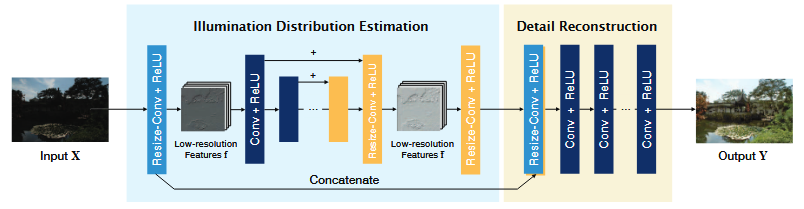
\includegraphics[width=0.8\columnwidth]{GLADNet}
%					
%					\begin{subfigure}{0.3\textwidth}
%						\includegraphics[width=\linewidth]{picture/Clear sky}
%						\captionsetup{font=scriptsize}
%						\caption{Clear sky}
%						\label{fig: Clear sky}
%					\end{subfigure}
%					\begin{subfigure}{0.3\textwidth}
%						\includegraphics[width=\linewidth]{picture/Drizzle}
%						\captionsetup{font=scriptsize}
%						\caption{Drizzle}
%						\label{fig: Drizzle}
%					\end{subfigure}
%					\begin{subfigure}{0.3\textwidth}
%						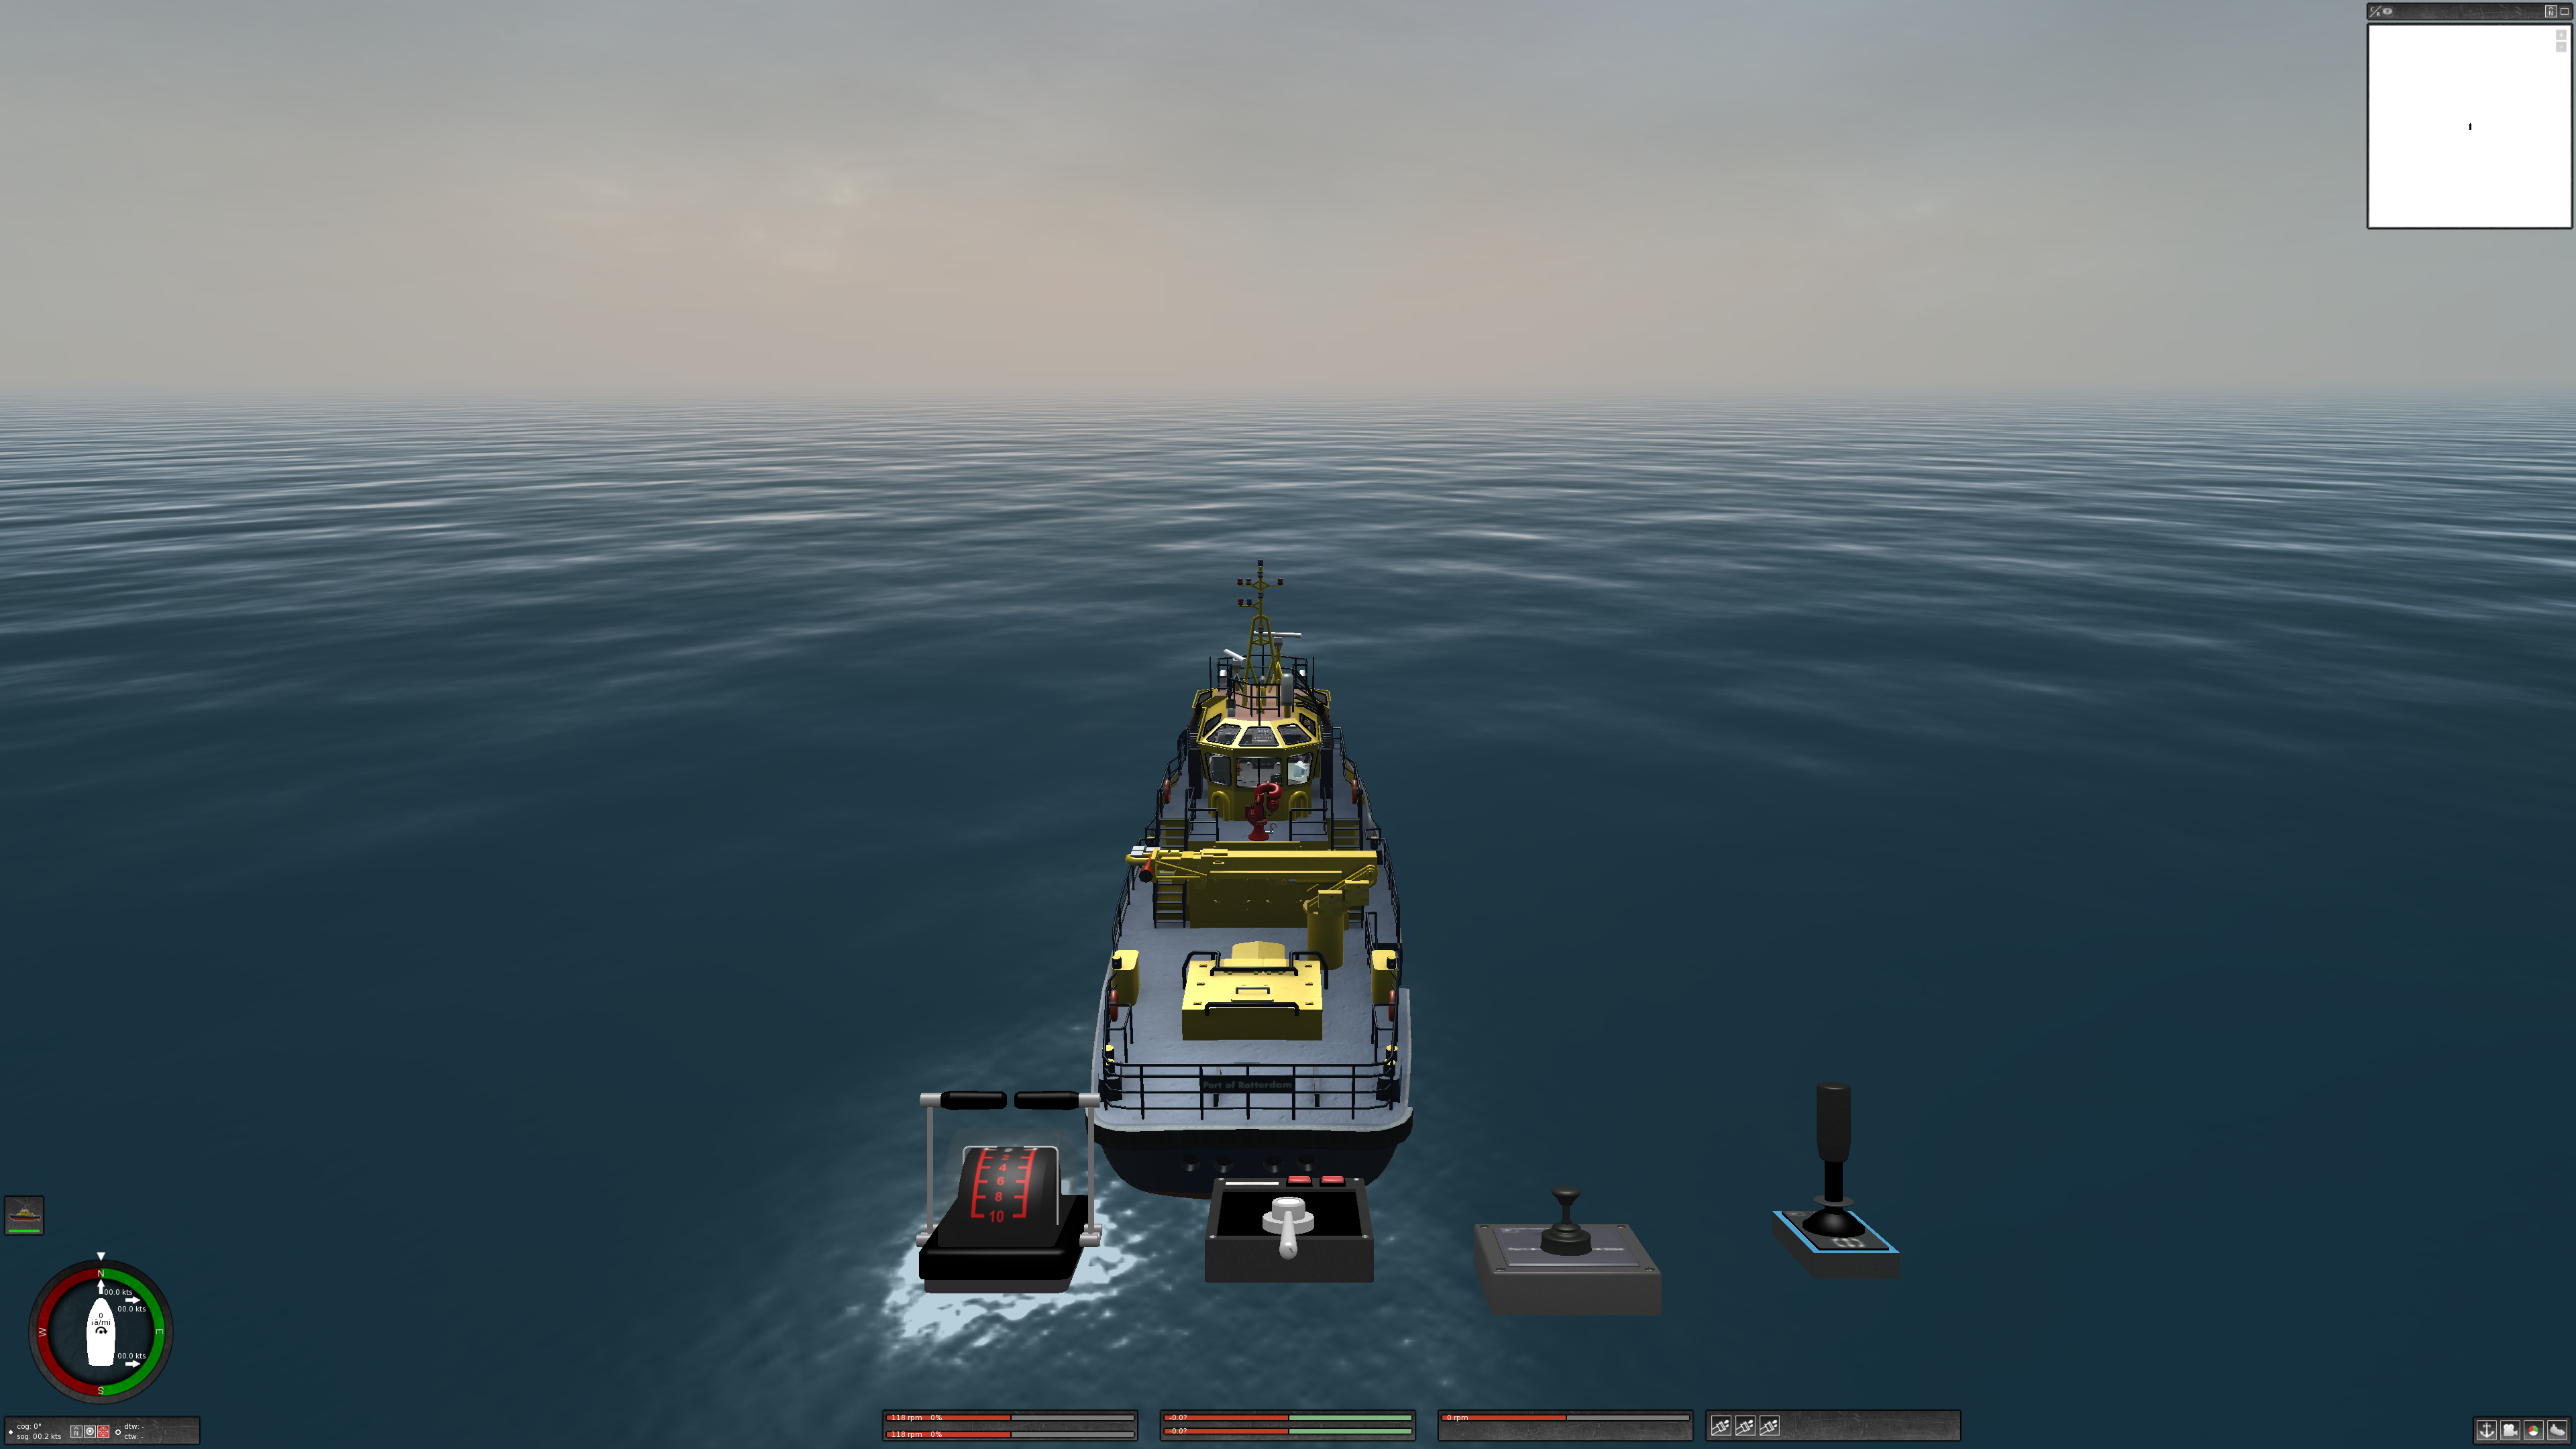
\includegraphics[width=\linewidth]{picture/Foggy}
%						\captionsetup{font=scriptsize}
%						\caption{Foggy}
%						\label{fig: Foggy}	
%					\end{subfigure}\\
%					\begin{subfigure}{0.3\textwidth}
%						\includegraphics[width=\linewidth]{picture/Hail}
%						\captionsetup{font=scriptsize}
%						\caption{Hail}
%						\label{fig: Hail}	
%					\end{subfigure}
%					\begin{subfigure}{0.3\textwidth}
%						\includegraphics[width=\linewidth]{picture/Light snow}
%						\captionsetup{font=scriptsize}
%						\caption{Light snow}
%						\label{fig: Light snow}
%					\end{subfigure}
%					\begin{subfigure}{0.3\textwidth}
%						\includegraphics[width=\linewidth]{picture/Rainy}
%						\captionsetup{font=scriptsize}
%						\caption{Rainy}
%						\label{fig: Rainy}
%					\end{subfigure}\\
%					\begin{subfigure}{0.3\textwidth}
%						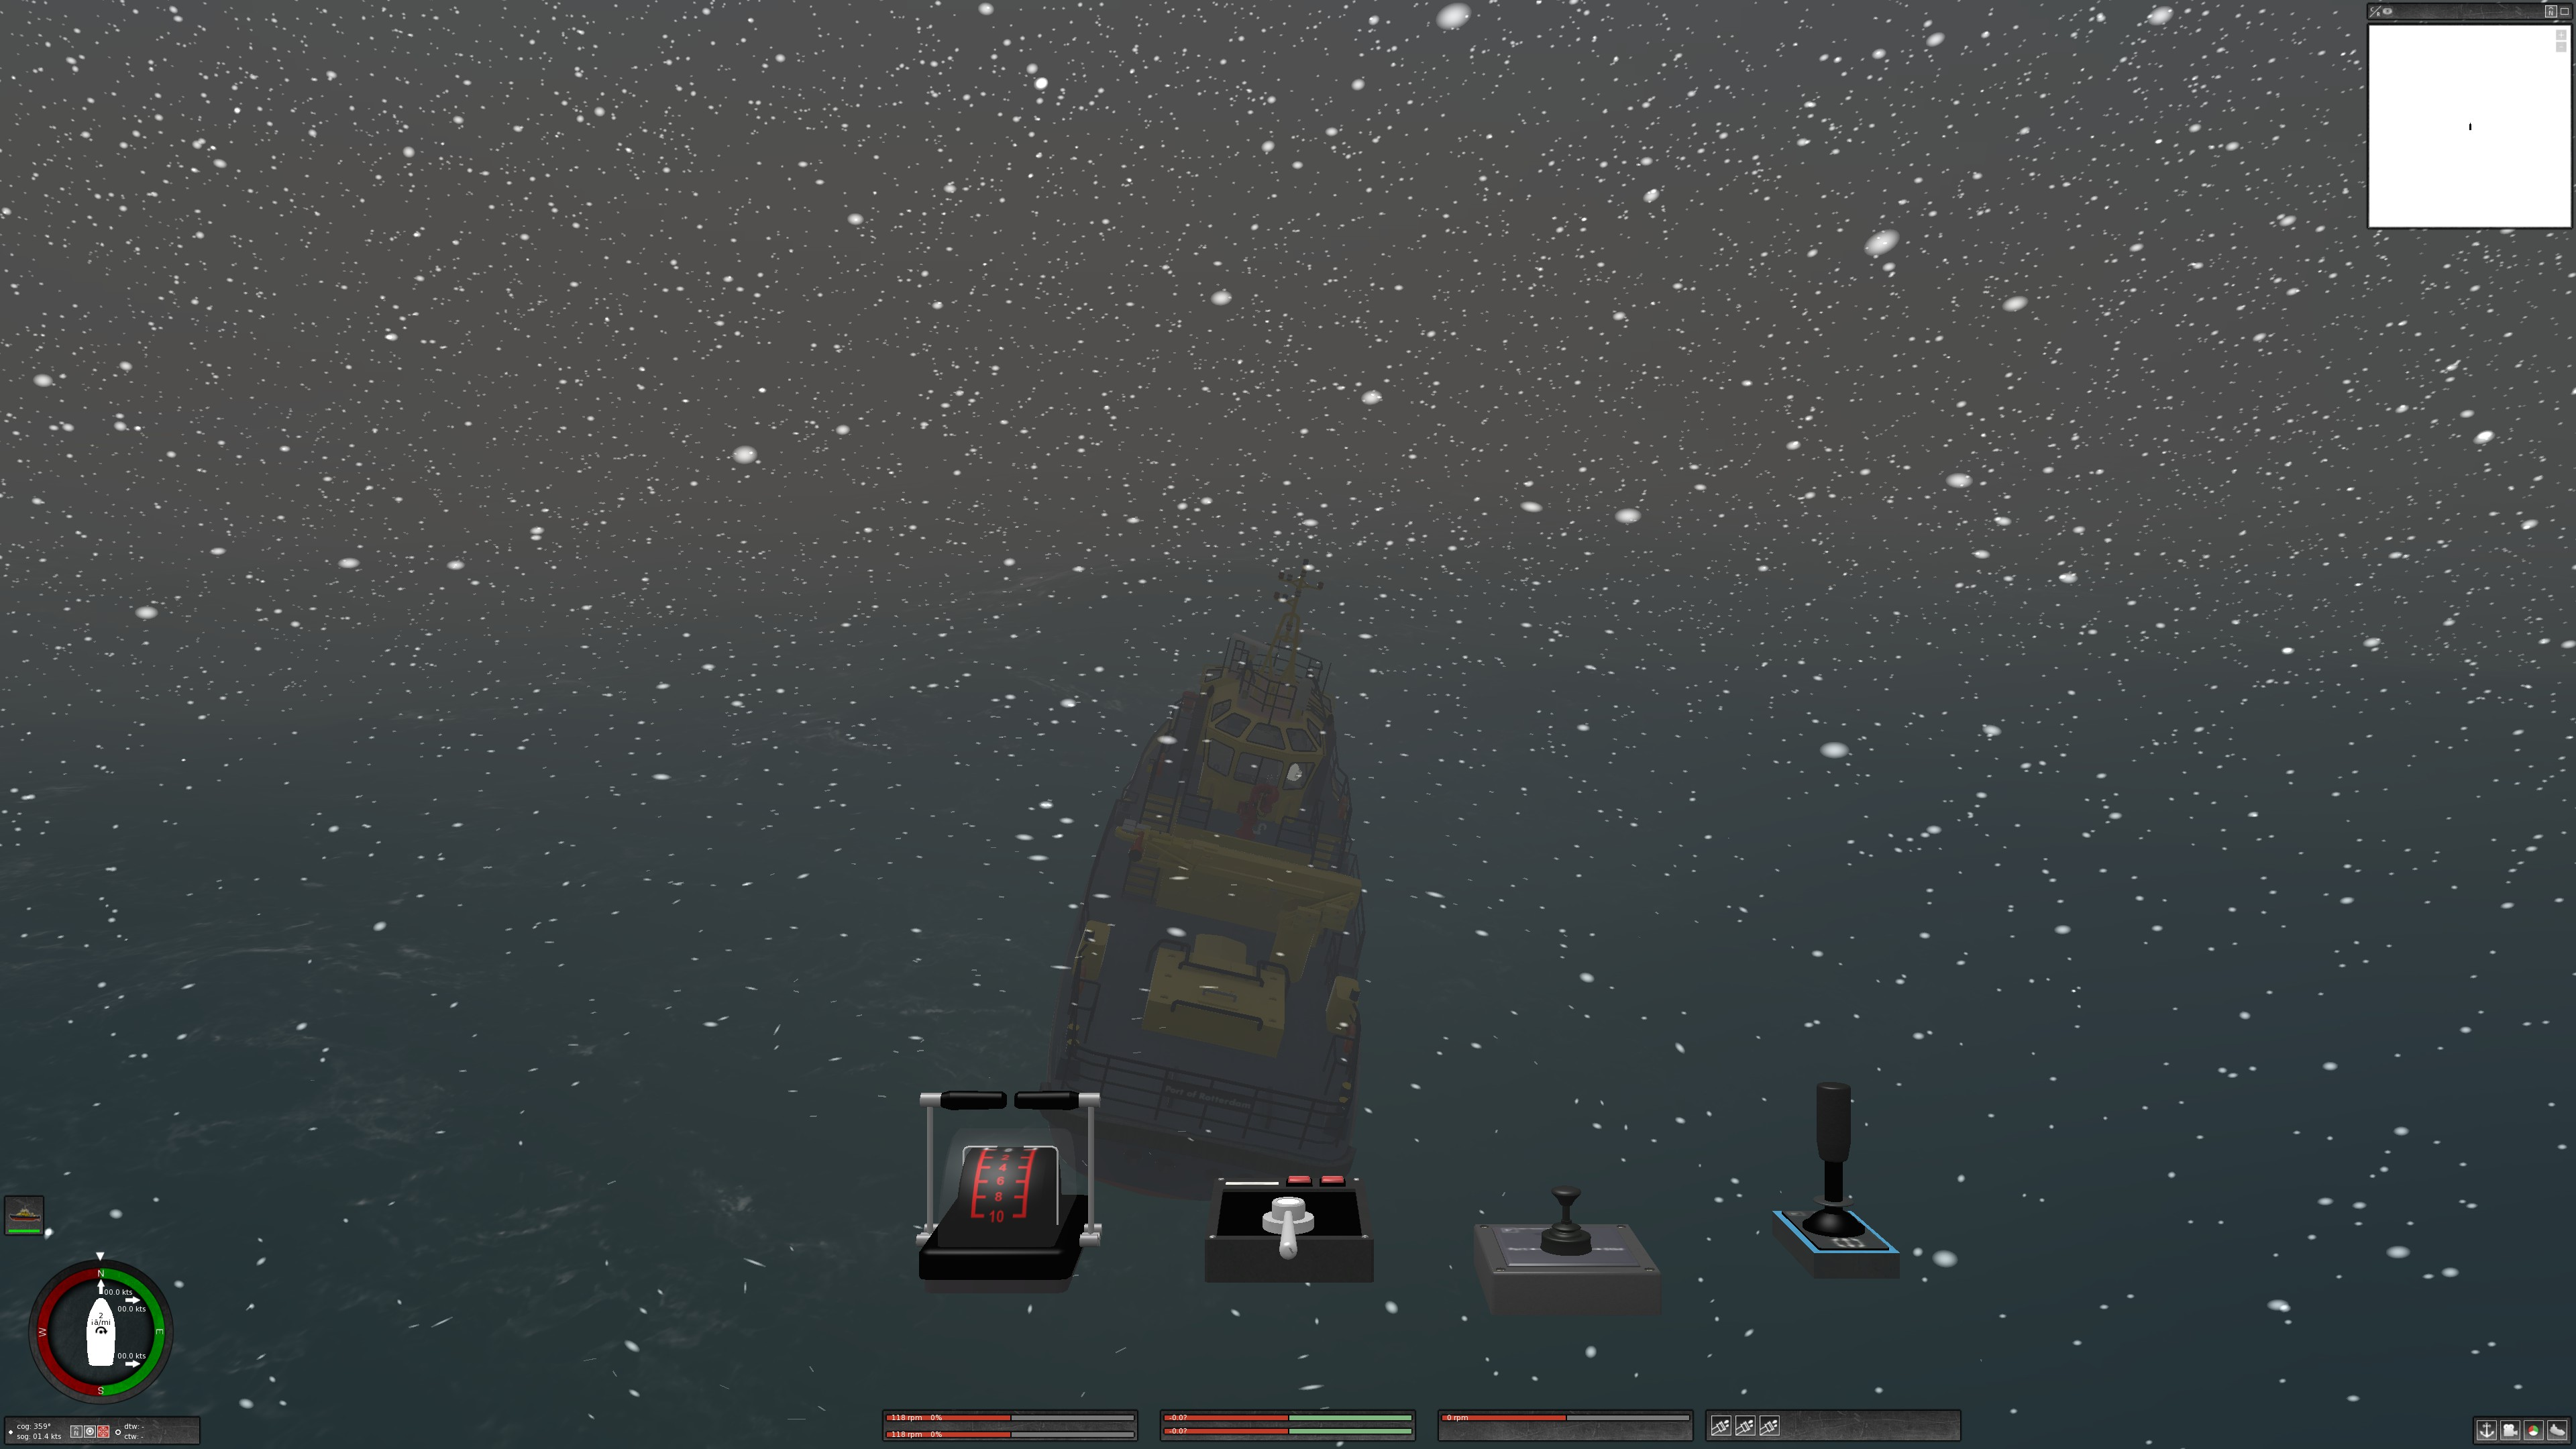
\includegraphics[width=\linewidth]{picture/Snow storm}
%						\captionsetup{font=scriptsize}
%						\caption{Snow storm}
%						\label{fig: Snow storm}	
%					\end{subfigure}
%					\begin{subfigure}{0.3\textwidth}
%						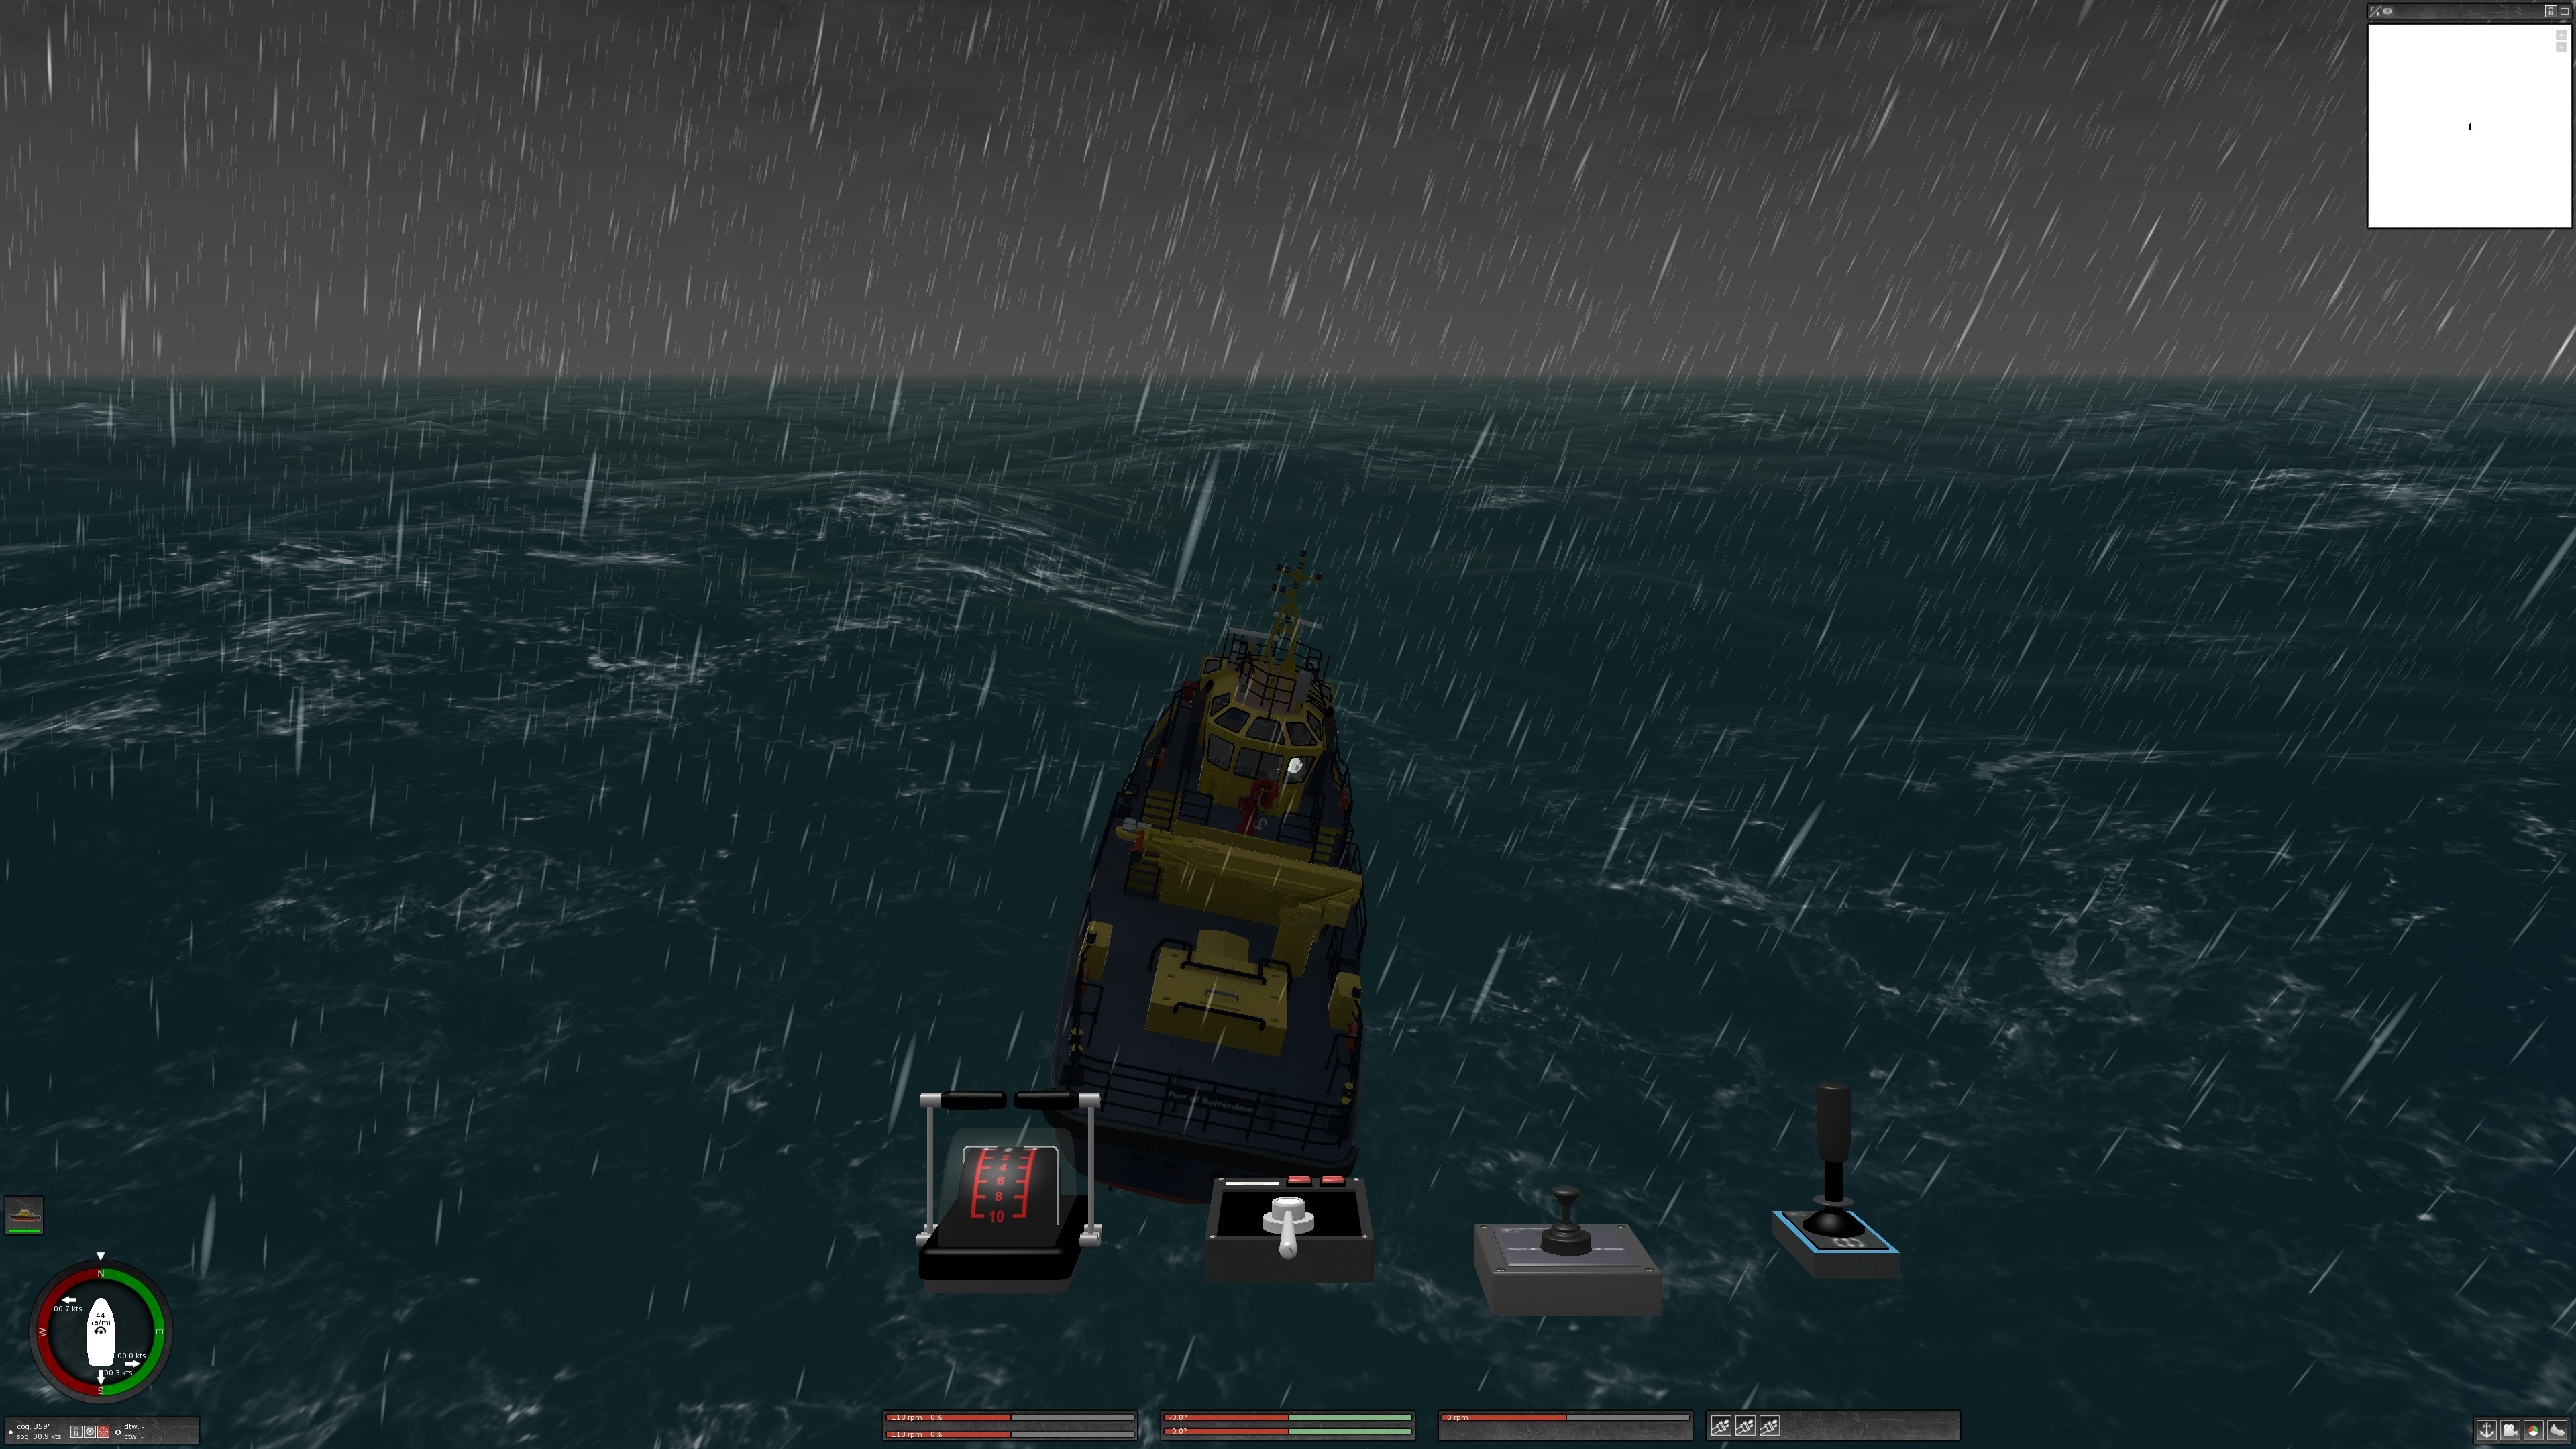
\includegraphics[width=\linewidth]{picture/Storm}
%						\captionsetup{font=scriptsize}
%						\caption{Storm}
%						\label{fig: Storm}	
%					\end{subfigure}
%					\begin{subfigure}{0.3\textwidth}
%						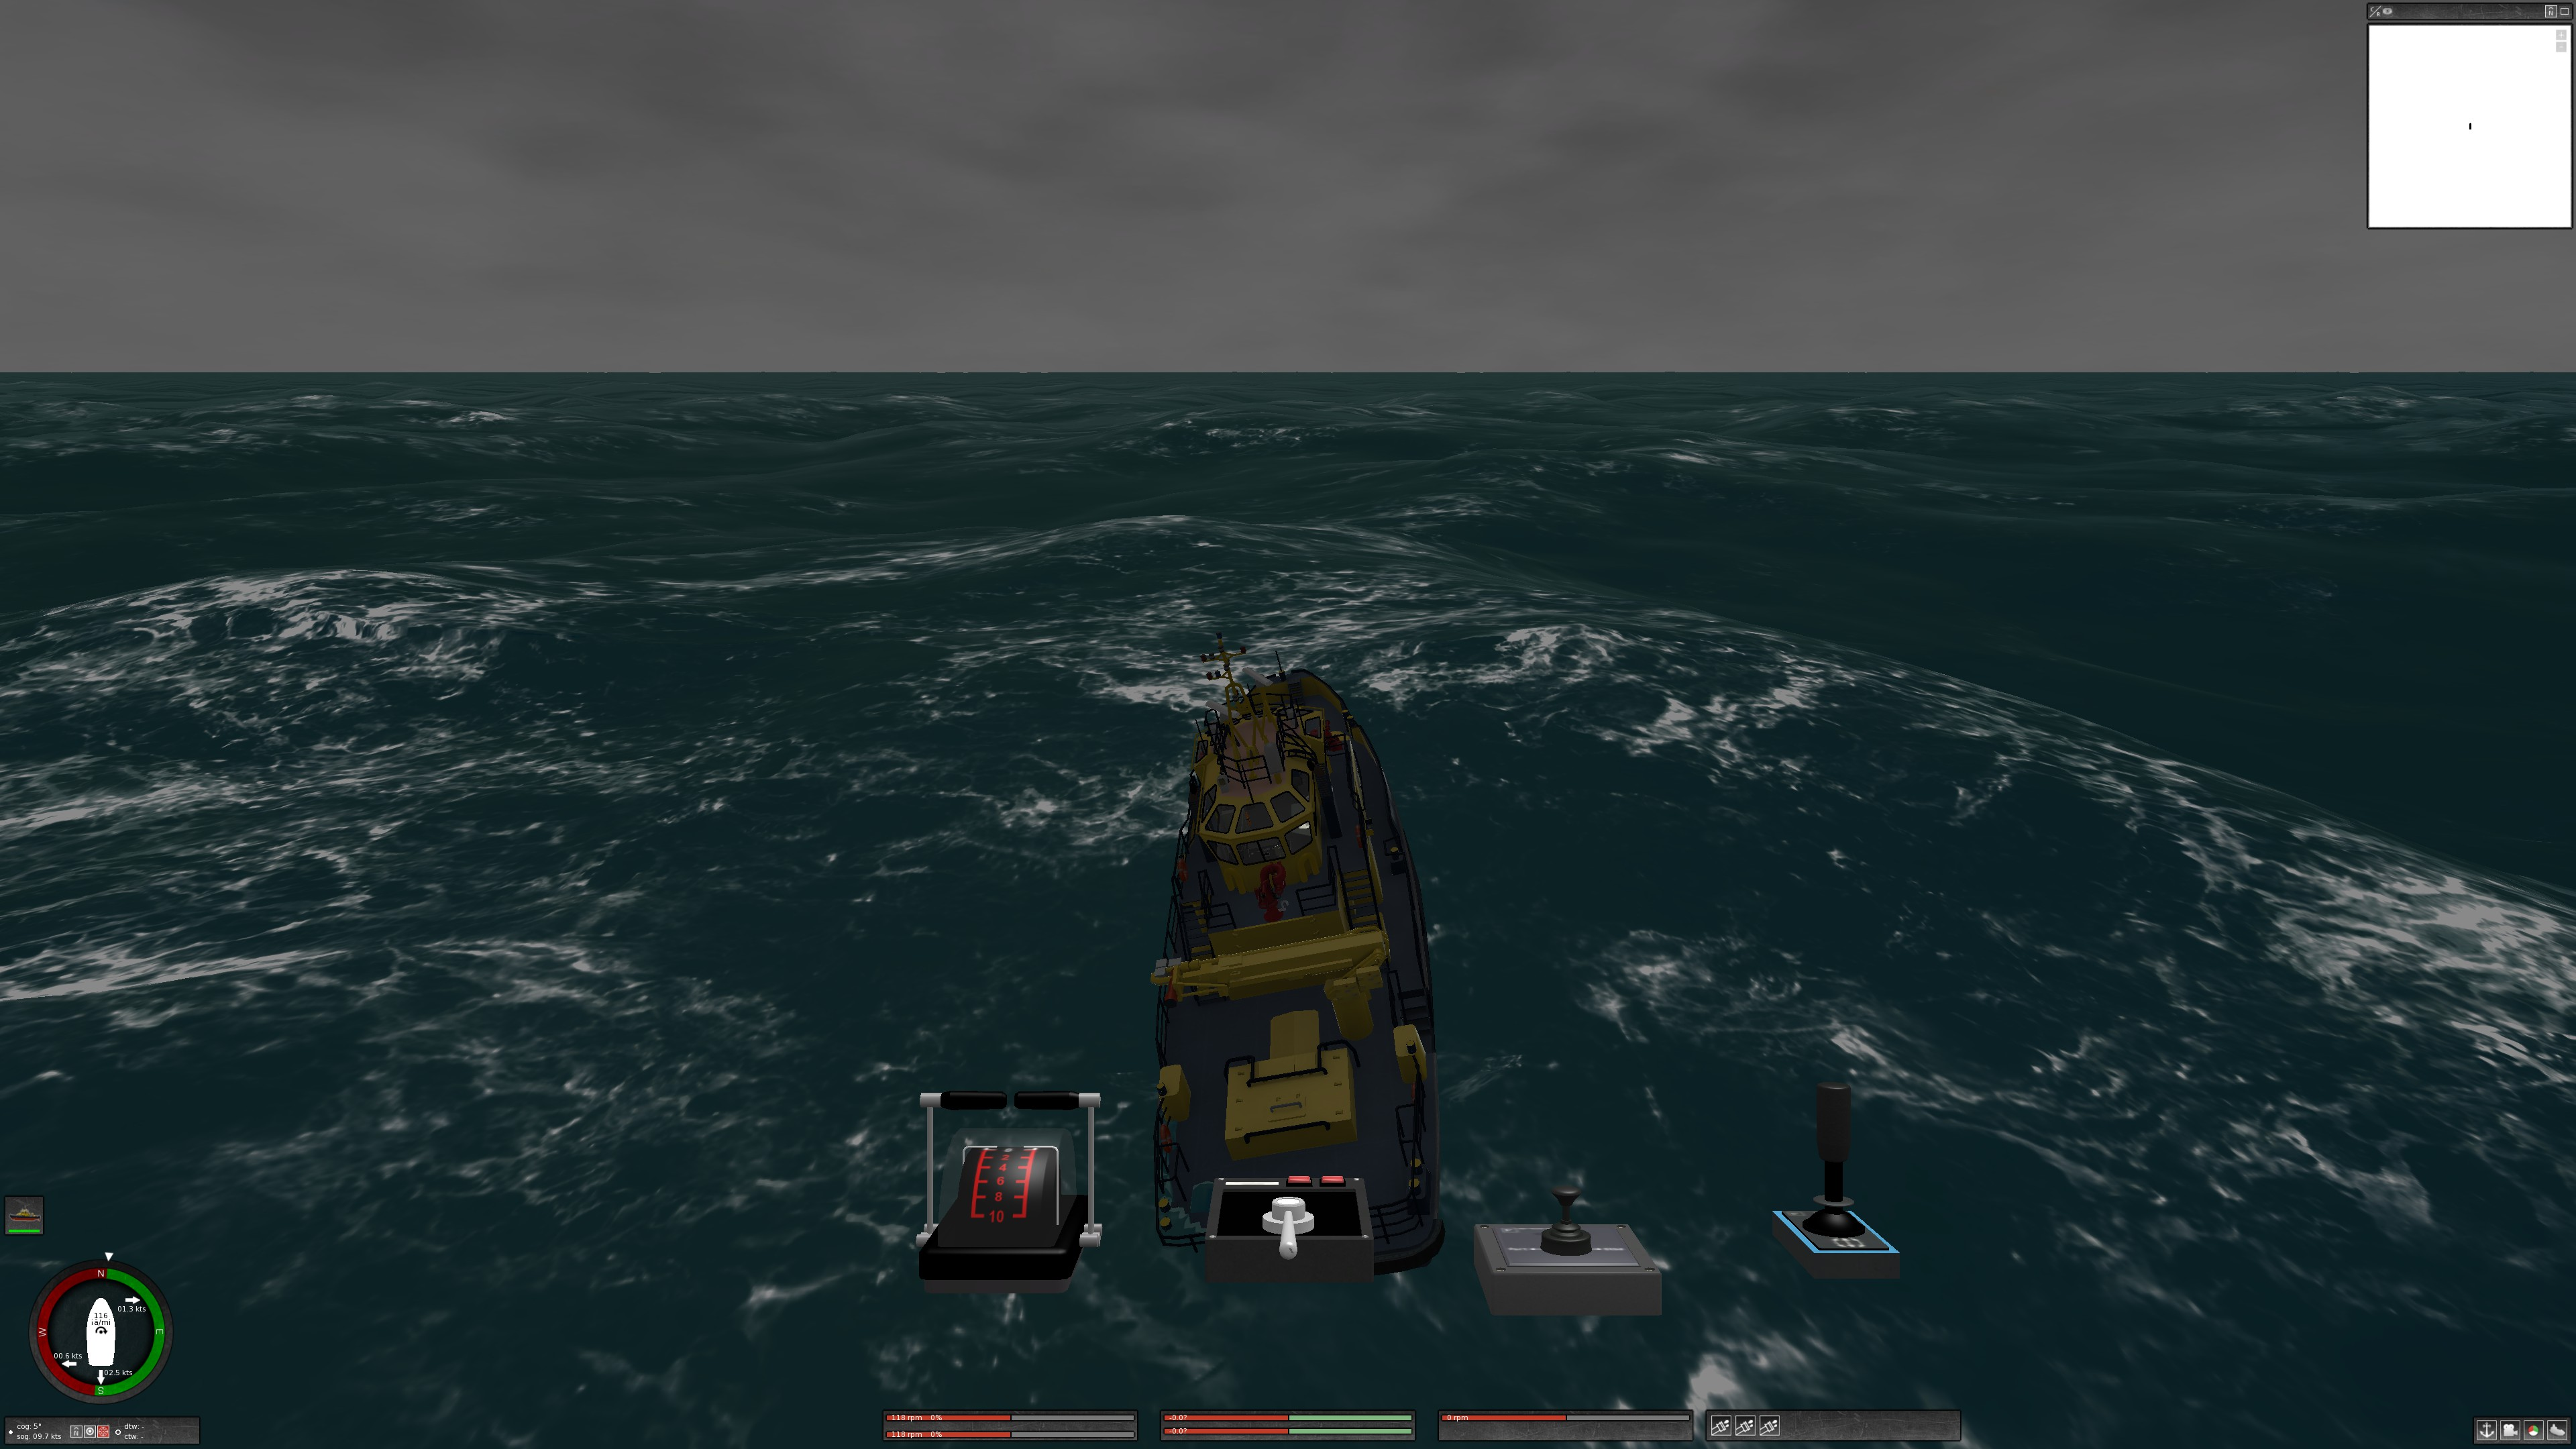
\includegraphics[width=\linewidth]{picture/Wind}
%						\captionsetup{font=scriptsize}
%						\caption{Wind}
%						\label{fig: Wind}
%					\end{subfigure}
%					\captionsetup{font=scriptsize}
%					\caption{
%						\label{fig: Weather}
%						9种不同的天气下的海况表现。
%					}
%				\end{figure}
%			
%				\paragraph{操作视角自定义}
%				
%				玩家在操纵船只时,可以自定义不同的操作视角,主要有三种游戏视角,一个自由视角,分别为 orbit(航线视角), helmsman(舵手视角), walkthrough(行人视角), photo camera mode, 如Fig. \ref{fig: View}所示。
%				
%				\begin{figure}[htbp] 
%					% read manual to see what [ht] means and for other possible options
%					\centering 
%					% 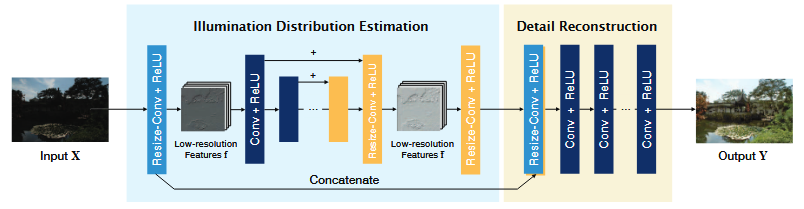
\includegraphics[width=0.8\columnwidth]{GLADNet}
%					
%					\begin{subfigure}{0.45\textwidth}
%						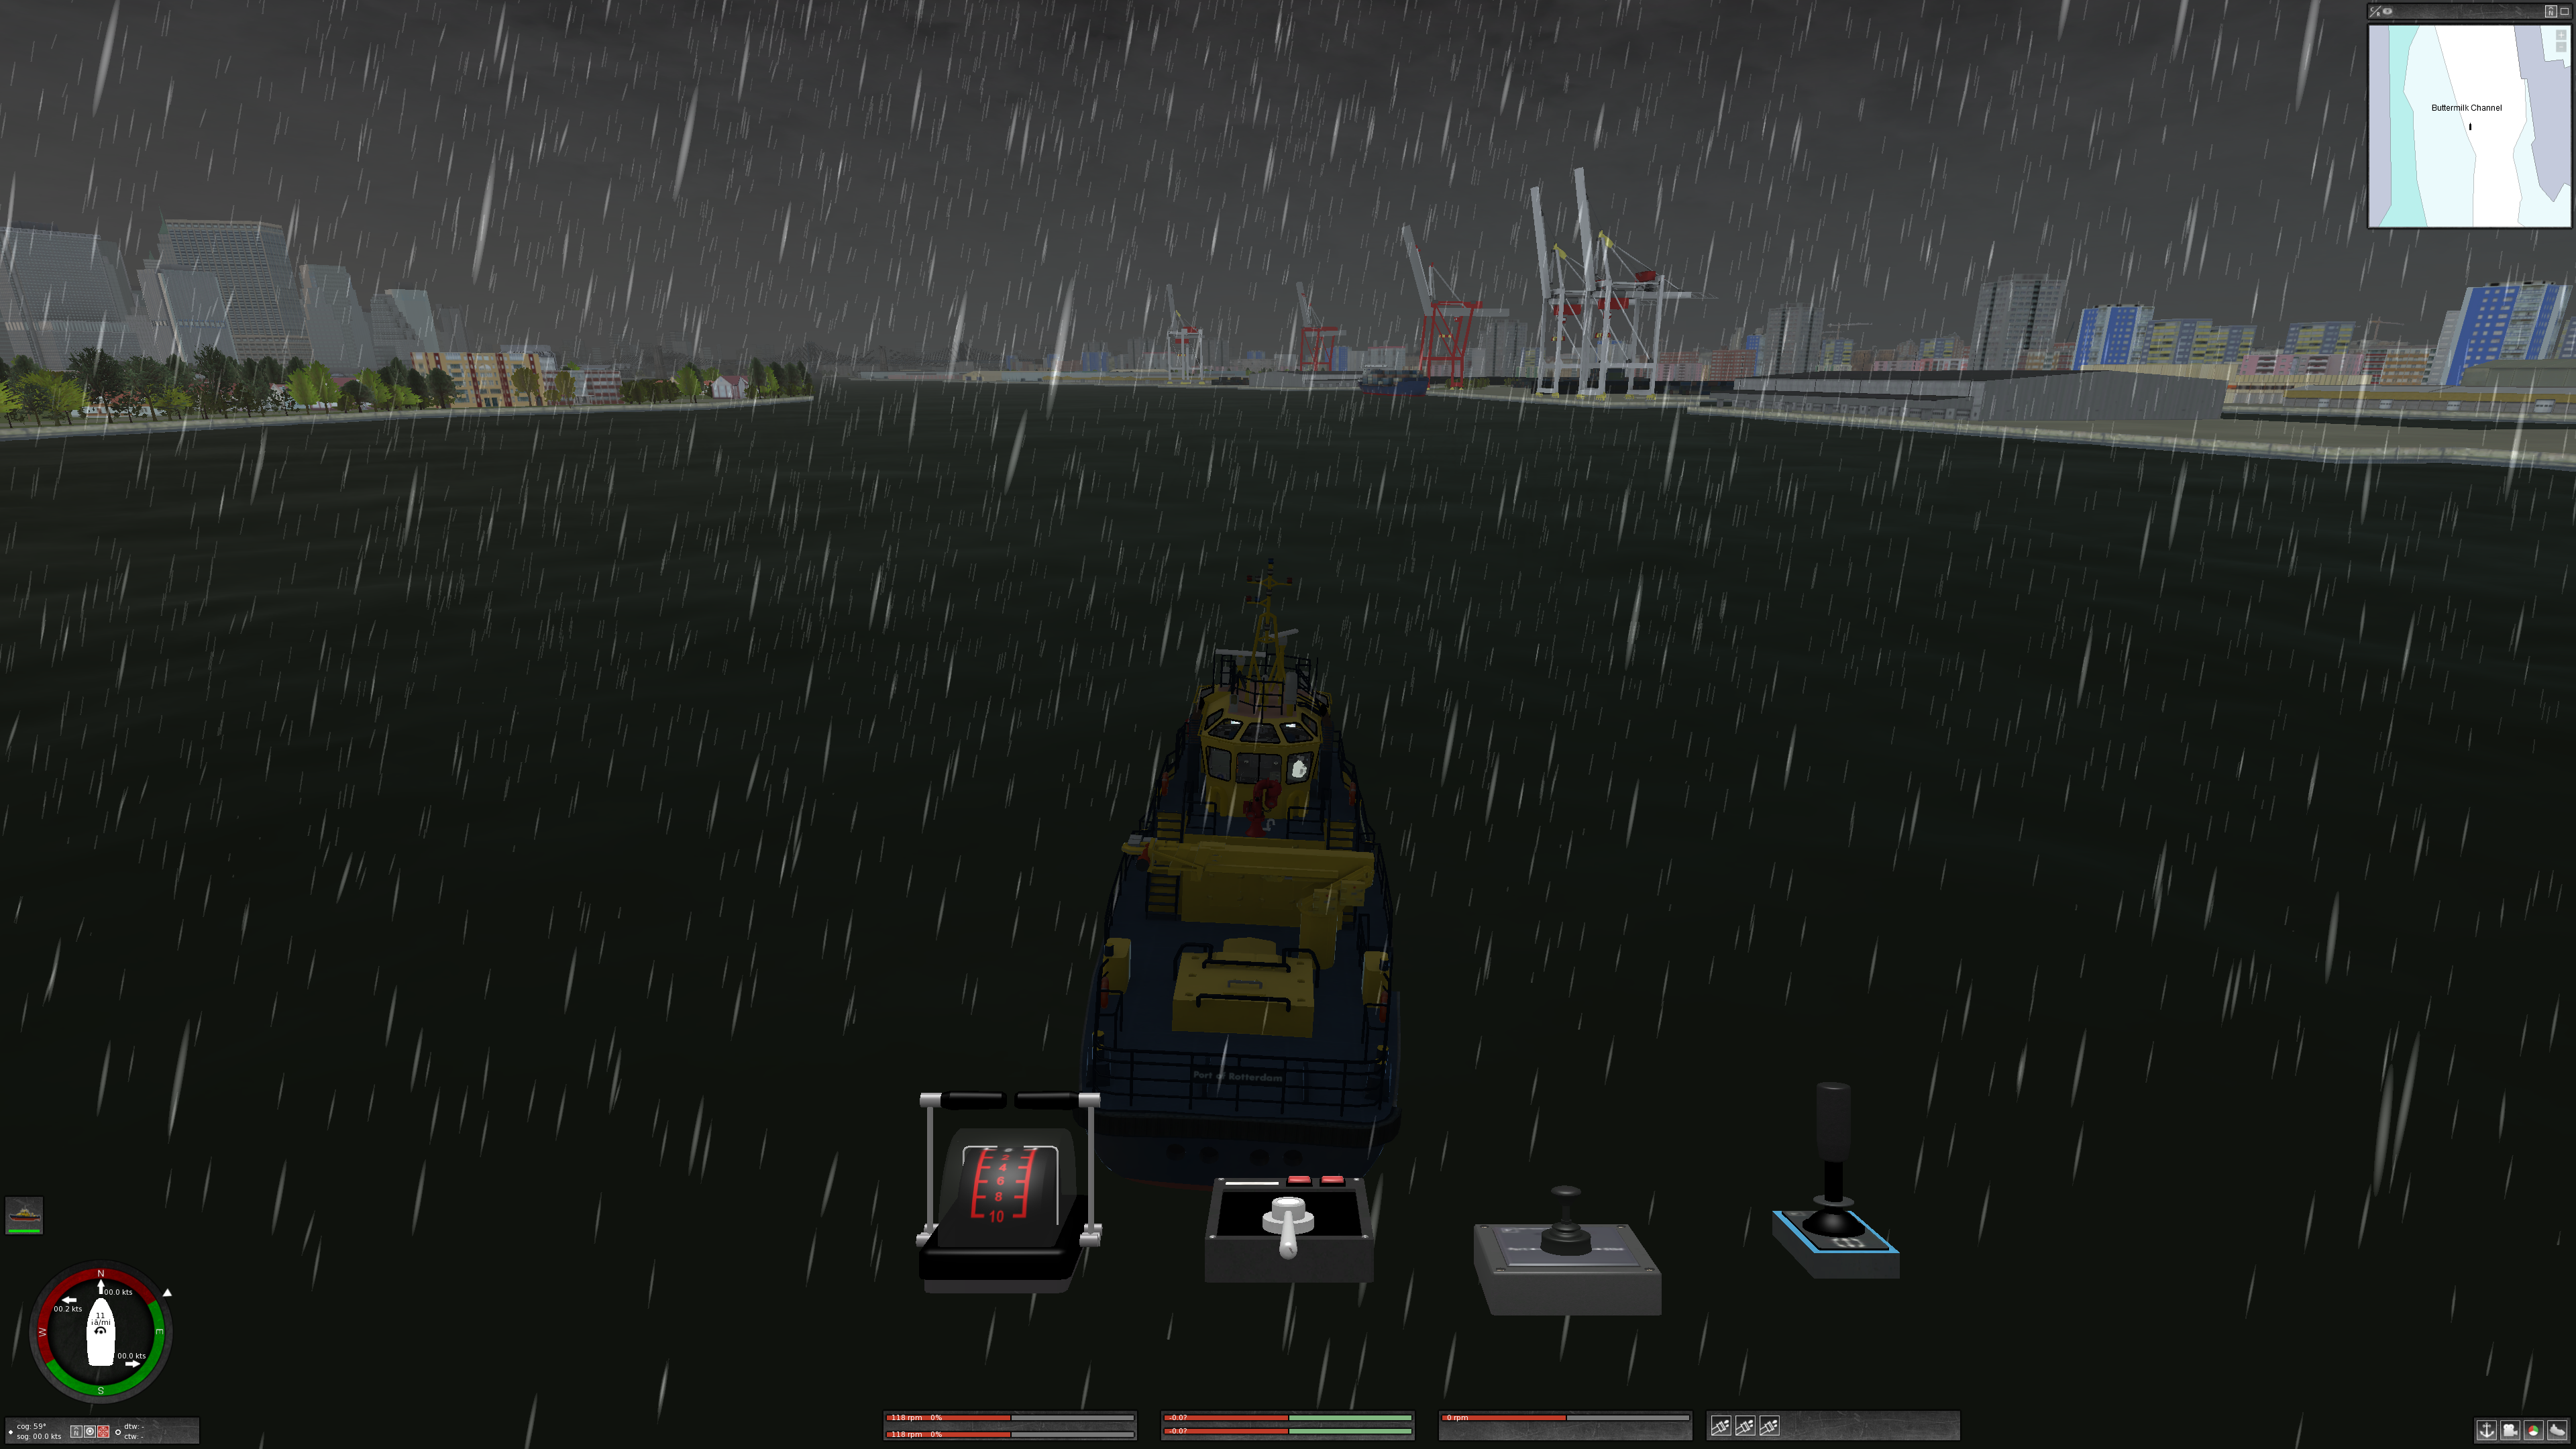
\includegraphics[width=\linewidth]{picture/orbit}
%						\captionsetup{font=scriptsize}
%						\caption{orbit}
%						\label{fig: orbit}
%					\end{subfigure}
%					\begin{subfigure}{0.45\textwidth}
%						\includegraphics[width=\linewidth]{picture/helmsman}
%						\captionsetup{font=scriptsize}
%						\caption{Drizzle}
%						\label{fig: helmsman}
%					\end{subfigure}\\
%					\begin{subfigure}{0.45\textwidth}
%						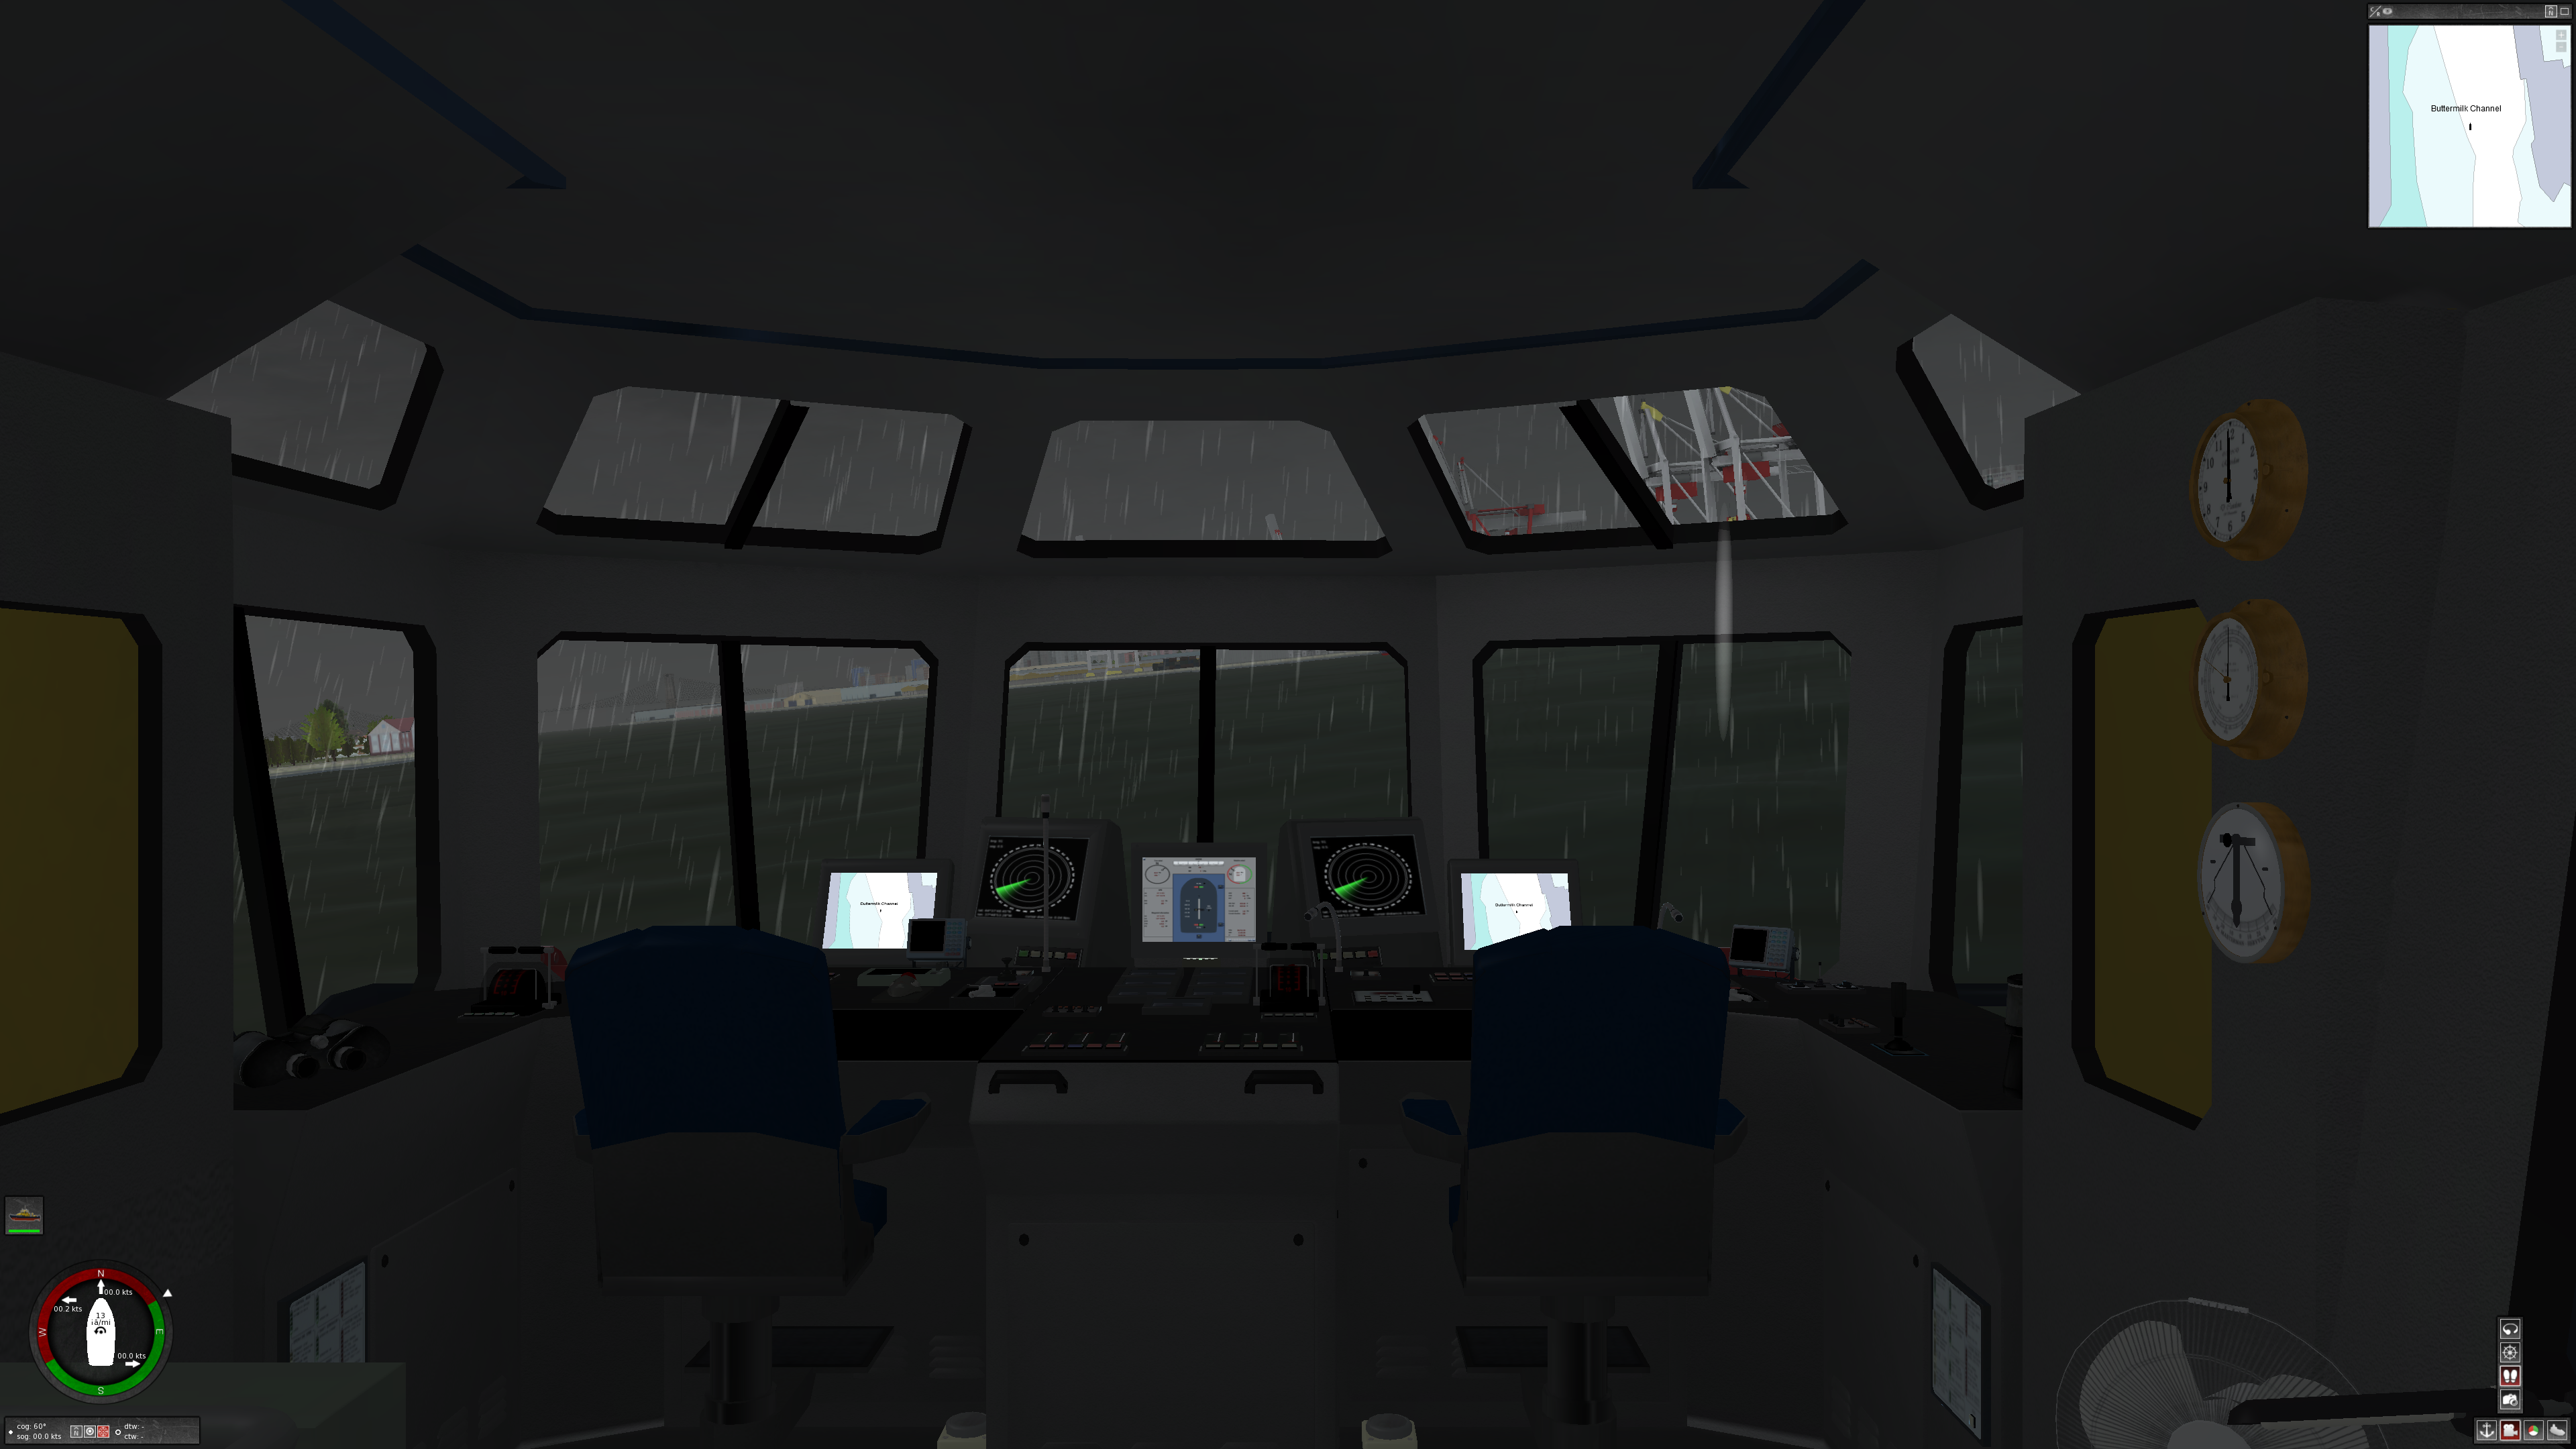
\includegraphics[width=\linewidth]{picture/walkthrough}
%						\captionsetup{font=scriptsize}
%						\caption{Walkthrough}
%						\label{fig: walkthrough}	
%					\end{subfigure}
%					\begin{subfigure}{0.45\textwidth}
%						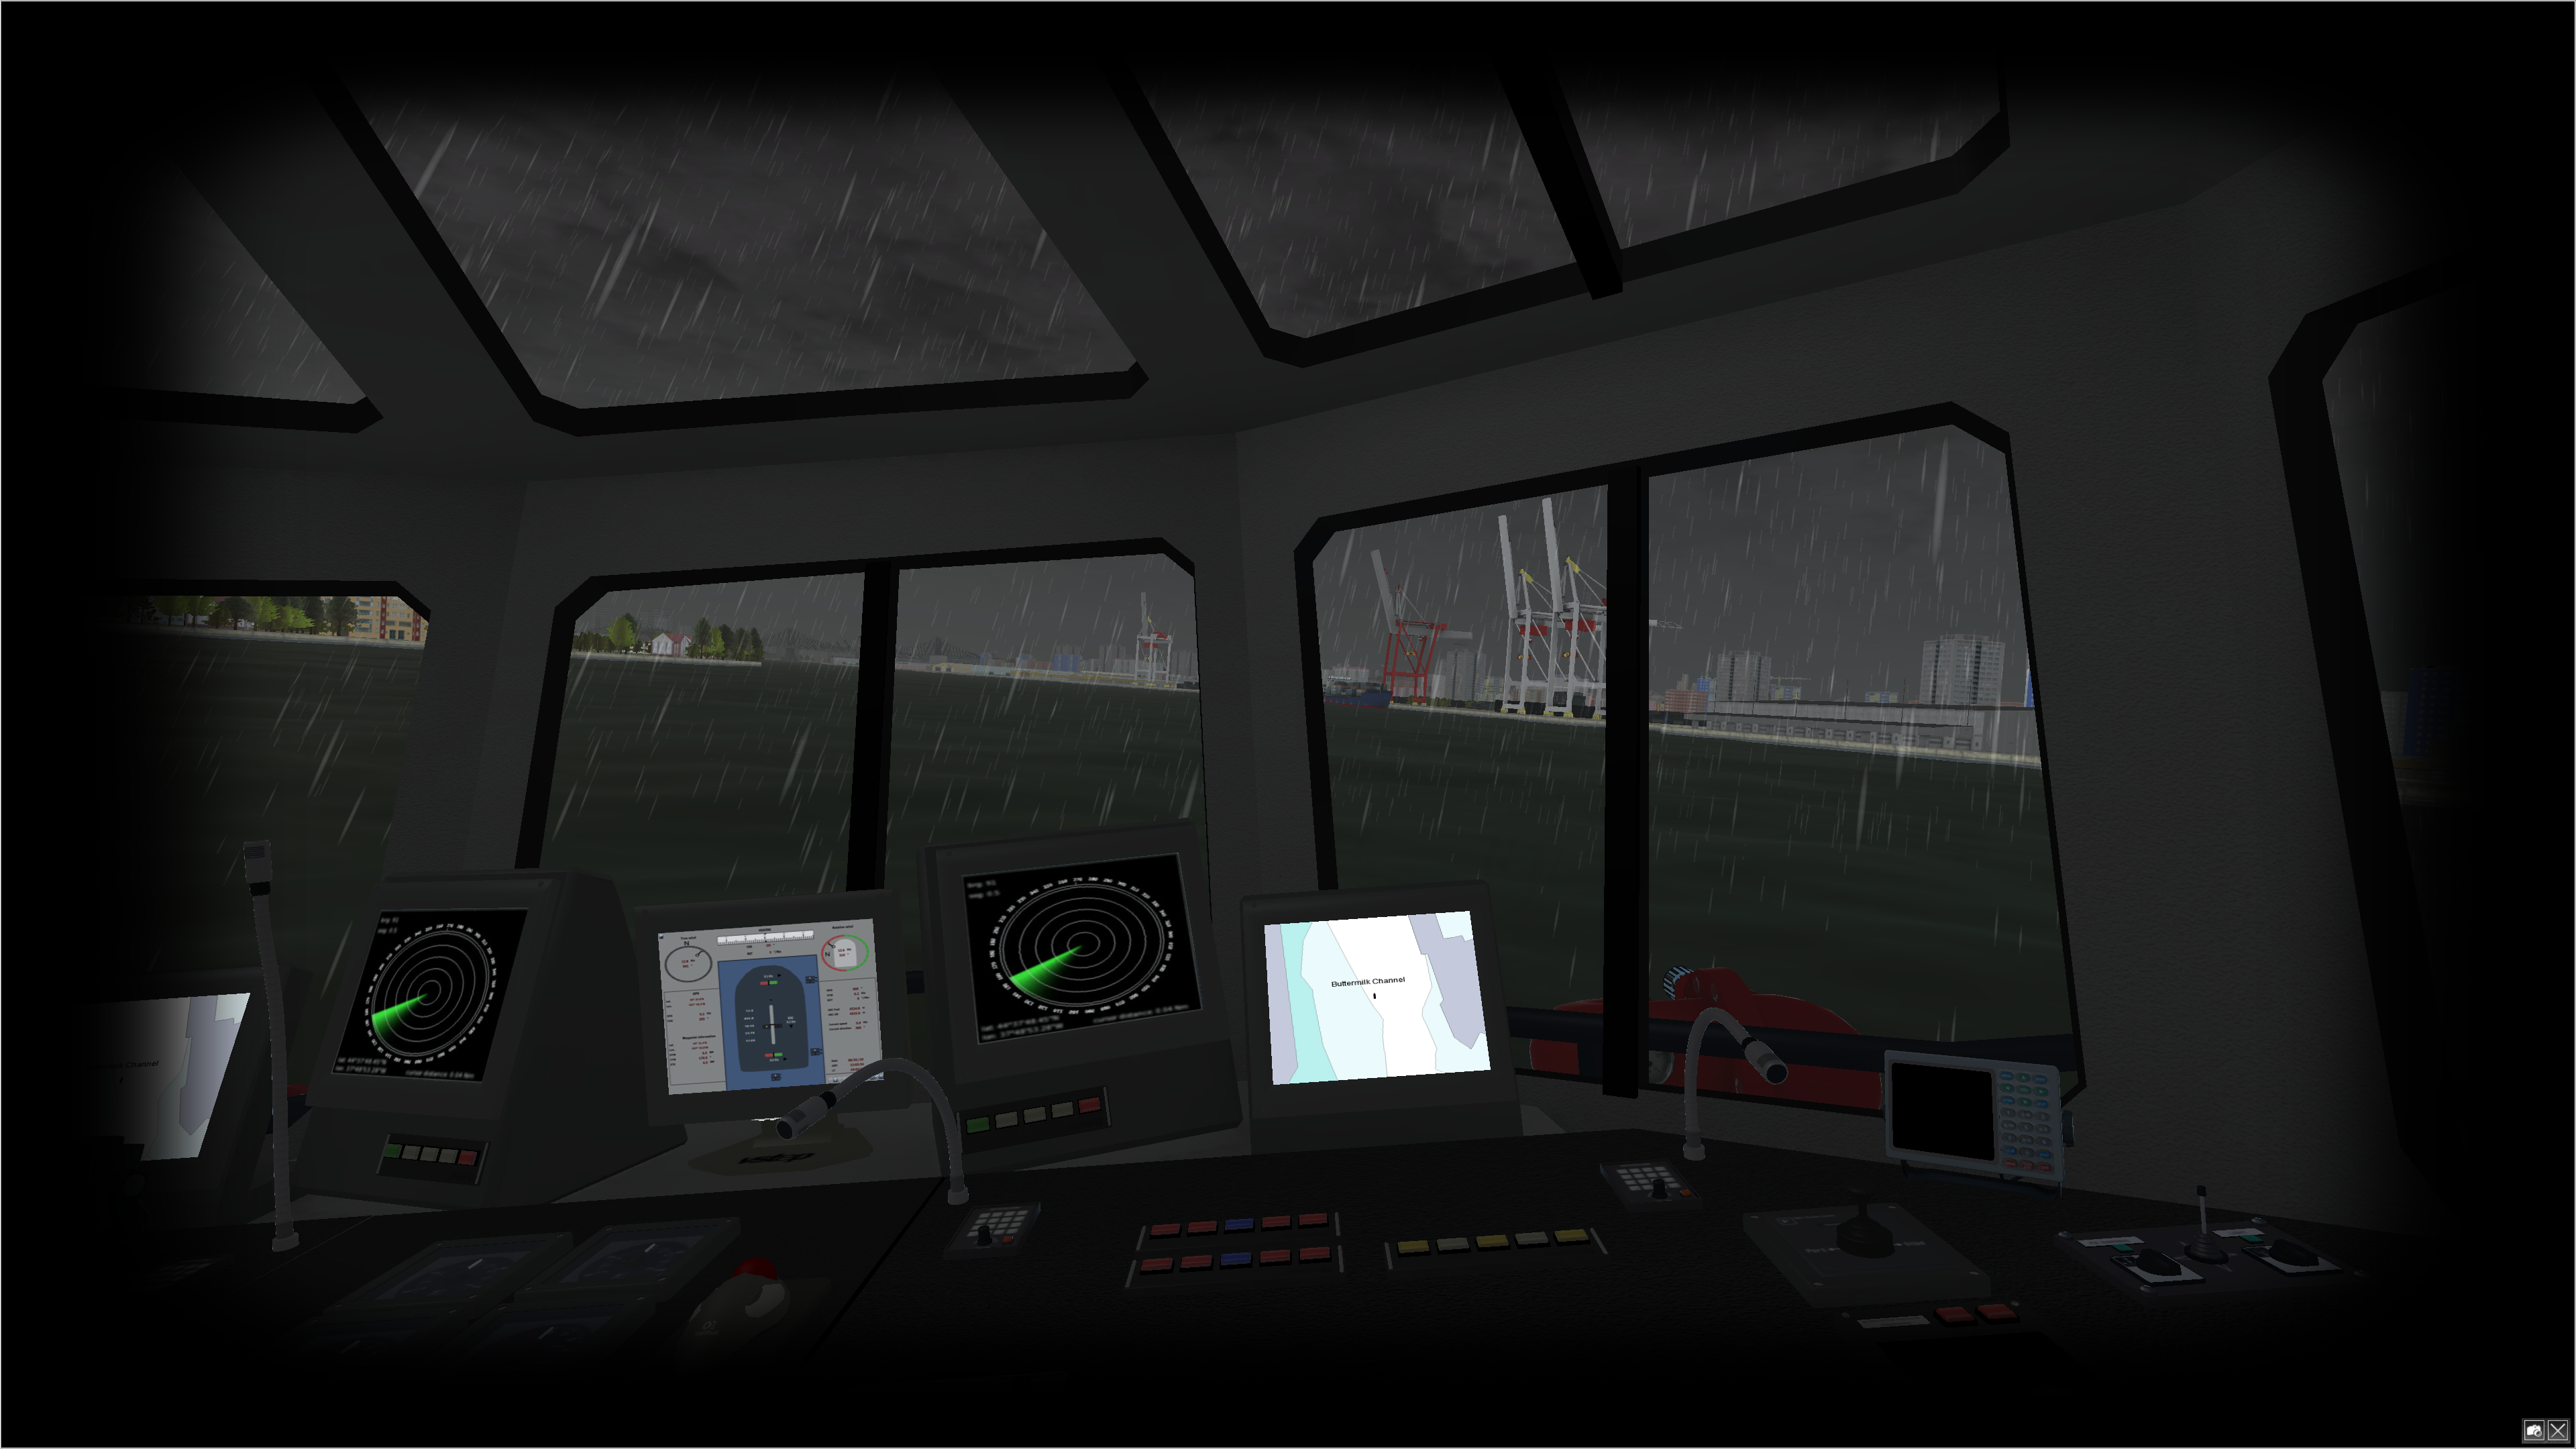
\includegraphics[width=\linewidth]{picture/photo camera mode}
%						\captionsetup{font=scriptsize}
%						\caption{photo camera mode}
%						\label{fig: photo camera mode}	
%					\end{subfigure}
%					\captionsetup{font=scriptsize}
%					\caption{
%						\label{fig: View}						
%						4种不同的操控视角。
%					}
%				\end{figure}

	%	\section{Analysis}
	
	%	In this section you will need to show your experimental results. Use tables and
	%	graphs when it is possible. Table~\ref{tbl:bins} is an example.
	
	%	\begin{table}[ht]
		%		\begin{center}
			%			\caption{Every table needs a caption.}
			%			\label{tbl:bins} % spaces are big no-no withing labels
			%			\begin{tabular}{|ccc|} 
				%				\hline
				%				\multicolumn{1}{|c}{$x$ (m)} & \multicolumn{1}{c|}{$V$ (V)} & \multicolumn{1}{c|}{$V$ (V)} \\
				%				\hline
				%				0.0044151 &   0.0030871 &   0.0030871\\
				%				0.0021633 &   0.0021343 &   0.0030871\\
				%				0.0003600 &   0.0018642 &   0.0030871\\
				%				0.0023831 &   0.0013287 &   0.0030871\\
				%				\hline
				%			\end{tabular}
			%		\end{center}
		%	\end{table}
	%	
	%	Analysis of equation~\ref{eq:aperp} shows ...
	%	
	%	Note: this section can be integrated with the previous one as long as you
	%	address the issue. Here explain how you determine uncertainties for different
	%	measured values. Suppose that in the experiment you make a series of
	%	measurements of a resistance of the wire $R$ for different applied voltages
	%	$V$, then you calculate the temperature from the resistance using a known
	%	equation and make a plot  temperature vs. voltage squared. Again suppose that
	%	this dependence is expected to be linear~\cite{Cyr}, and the proportionality coefficient
	%	is extracted from the graph. Then what you need to explain is that for the
	%	resistance and the voltage the uncertainties are instrumental (since each
	%	measurements in done only once), and they are $\dots$. Then give an equation
	%	for calculating the uncertainty of the temperature from the resistance
	%	uncertainty. Finally explain how the uncertainty of the slop of the graph was
	%	found (computer fitting, graphical method, \emph{etc}.)
	%	
	%	If in the process of data analysis you found any noticeable systematic
	%	error(s), you have to explain them in this section of the report.
	%	
	%	It is also recommended to plot the data graphically to efficiently illustrate
	%	any points of discussion. For example, it is easy to conclude that the
	%	experiment and theory match each other rather well if you look at
	%	Fig.~\ref{fig:samplesetup} and Fig.~\ref{fig:exp_plots}.
	%	
	%	\begin{figure}[ht] 
		%		\centering
		%		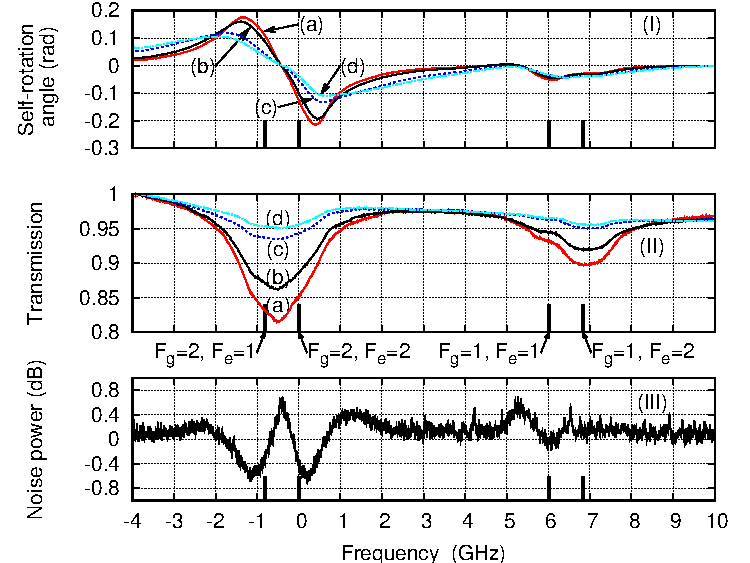
\includegraphics[width=0.5\columnwidth]{sr_squeezing_vs_detuning}
		%		
		%		% some figures do not need to be too wide
		%		\caption{
			%			\label{fig:exp_plots}  
			%			Every plot must have axes labeled.
			%		}
		%	\end{figure}
	
	
	%	\section{Conclusions}
	%	Here you briefly summarize your findings.
	
	%++++++++++++++++++++++++++++++++++++++++
	% References section will be created automatically 
	% with inclusion of "thebibliography" environment
	% as it shown below. See text starting with line
	% \begin{thebibliography}{99}
		% Note: with this approach it is YOUR responsibility to put them in order
		% of appearance.
		
		\renewcommand{\refname}{References}
		
		
		%	\begin{thebibliography}{00}
			
			%		\bibitem{b1}\label{cite:b1}
			%		W. Wang, C. Wei, W. Yang and J. Liu, "GLADNet: Low-Light Enhancement Network with Global Awareness," 2018 13th IEEE International Conference on Automatic Face \& Gesture Recognition (FG 2018), Xi'an, China, 2018, pp. 751-755, DOI: 10.1109/FG.2018.00118.
			
			%		\bibitem{b2}\label{cite:b2}
			%		A.\ Mahajan, K.\ Somaraj and M. Sameer, "Adopting Artificial Intelligence Powered ConvNet To Detect Epileptic Seizures," 2020 IEEE-EMBS Conference on Biomedical Engineering and Sciences (IECBES), Langkawi Island, Malaysia, 2021, pp. 427-432, DOI: 10.1109/IECBES48179.2021.9398832.
			
			%		\bibitem{Cyr}
			%		N.\ Cyr, M.\ T$\hat{e}$tu, and M.\ Breton,
			% "All-optical microwave frequency standard: a proposal,"
			%		IEEE Trans.\ Instrum.\ Meas.\ \textbf{42}, 640 (1993).
			
			
			
			%	\end{thebibliography}
		
		\bibliographystyle{unsrt}
		\bibliography{reference}
		
		
	\end{document}
